% !TEX root = Tesi.tex
\chead{}

\chapter{Enhancing web models via model transformations}
\label{enhancing-web-models-via-model-transformations}

\section{Transformation}

In the previous chapter, after describing both metamodels for the Real Usage Data and the Interaction Flow Modeling Language, we proceeded with creating dynamic instances for both models, respectively describing the actual input data available for the customisation process and the initial IFMLModel of the eCommerce Madison Island website. In this chapter, we illustrate a possible transformation for this model, based on the Real Usage instance data. Our goal is to upgrade the model version, taking into account customers preferences and their actions.

\subsection{Homepage}
\label{homepage-updates}
Considering the data coming from the Proximity sensors within the actual Madison Island retail store, we are aware of a set of regions corresponding to the customer preferred categories. That information will be used to change the content and, therefore, the IFMLModel for the Homepage carousel.

For instance, we know that the \textbf{Blazers}, \textbf{Tees, Knits and Polos} and \textbf{Shoes} categories correspond to the \textit{sessionRegion} elements within the store in which the user spent more time after sorting the entries by \textit{maxSecondsInRegion} and \textit{maxProximity} attributes. In the case of the Blazers category for example, the data belonging to the \textit{RealUsageData:ProximityData} parent node takes this form:

\vspace{0.5cm}
\lstset{language=XML}
\begin{lstlisting} 
  <sessionRegions
  regionId="40"
  regionLabel="blazers"
  detectionCount="1"
  maxSecondsInRegion="195"
  maxProximity="immediate"
  firstDetectionTimeStamp="2018-02-21T18:11:01.000+0100"
  lastDetectionTimeStamp="2018-02-21T18:11:01.000+0100">
  <beaconData
    uuid="0686a88e-fed6-11e7-8be5-0ed5f89f718b"
    majorId="25911"
    minorId="27"/>
</sessionRegions>
\end{lstlisting}
\vspace{0.5cm}

By applying this knowledge, we can say that the \textit{subViewComponentParts} and the \textit{parameter} nodes of the first HightlightedCategoriesCarousel \textit{IFMLWindow} elements from the initial \textit{IFMLModel} can be modified from this:

\vspace{0.5cm}
\lstset{language=XML}
\begin{lstlisting} 
<parameters  name="Highlighted Category #1" direction="inout">
  <constraints  language="SQL" body="Category.ID=18"/>
</parameters>

...

<subViewComponentParts xsi:type="core:ConditionalExpression"  language="SQL" body="Category.ID=18" name="Eyewear"/>
\end{lstlisting}
\vspace{0.5cm}

to:

\vspace{0.5cm}
\lstset{language=XML}
\begin{lstlisting} 
  <parameters  name="Highlighted Category #1" direction="inout">
  <constraints  language="SQL" body="Category.ID=40"/>
</parameters>

...

<subViewComponentParts xsi:type="core:ConditionalExpression"  language="SQL" body="Category.ID=40" name="Blazers"/>
\end{lstlisting}
\vspace{0.5cm}

Besides updating the content by prioritising some categories, the \textit{IFMLModel} can also be changed to use different IFML elements under certain conditions. For example, the \textit{List View Component}, which is responsible for displaying the most recent products on the homepage, can be replaced by another \textit{List View Component}, responsible for presenting the latest products with which customers interacted in the physical store. Information about these products is available in the RealUsageData model under the \textit{RealUsageData:ActionData} section. In our specific example, \textit{RealUsageData:ActionData} contains the data about the product SKUs that the customer had scanned for collecting reward points.

\vspace{0.5cm}
\lstset{language=XML}
\begin{lstlisting} 
<sessionActions userAgent="iPhone 6S">
  <scannedItems 
  barcode="042100005264" name="Elizabeth Knit Top-Red-S" sku="wbk012c-Red-S"/>
  <scannedItems 
  barcode="042100005931" name="Plaid Cotton Shirt-Khaki-L" sku="msj006c-Khaki-L"/>
  <scannedItems 
  barcode="042100007717" name="Broad St Saddle Shoes" sku="shm00110"/>
</sessionActions>
\end{lstlisting}
\vspace{0.5cm}


The model transition in this case would occur not only replacing the IFML \textit{View Component} with a different type, but also adding a \textit{ConditionalExpression} that filters the items by their SKUs, as shown in Figure \ref{fig:ifml-transformation-example}.

\vspace{0.5cm}
\begin{figure}[H]
  \centering
    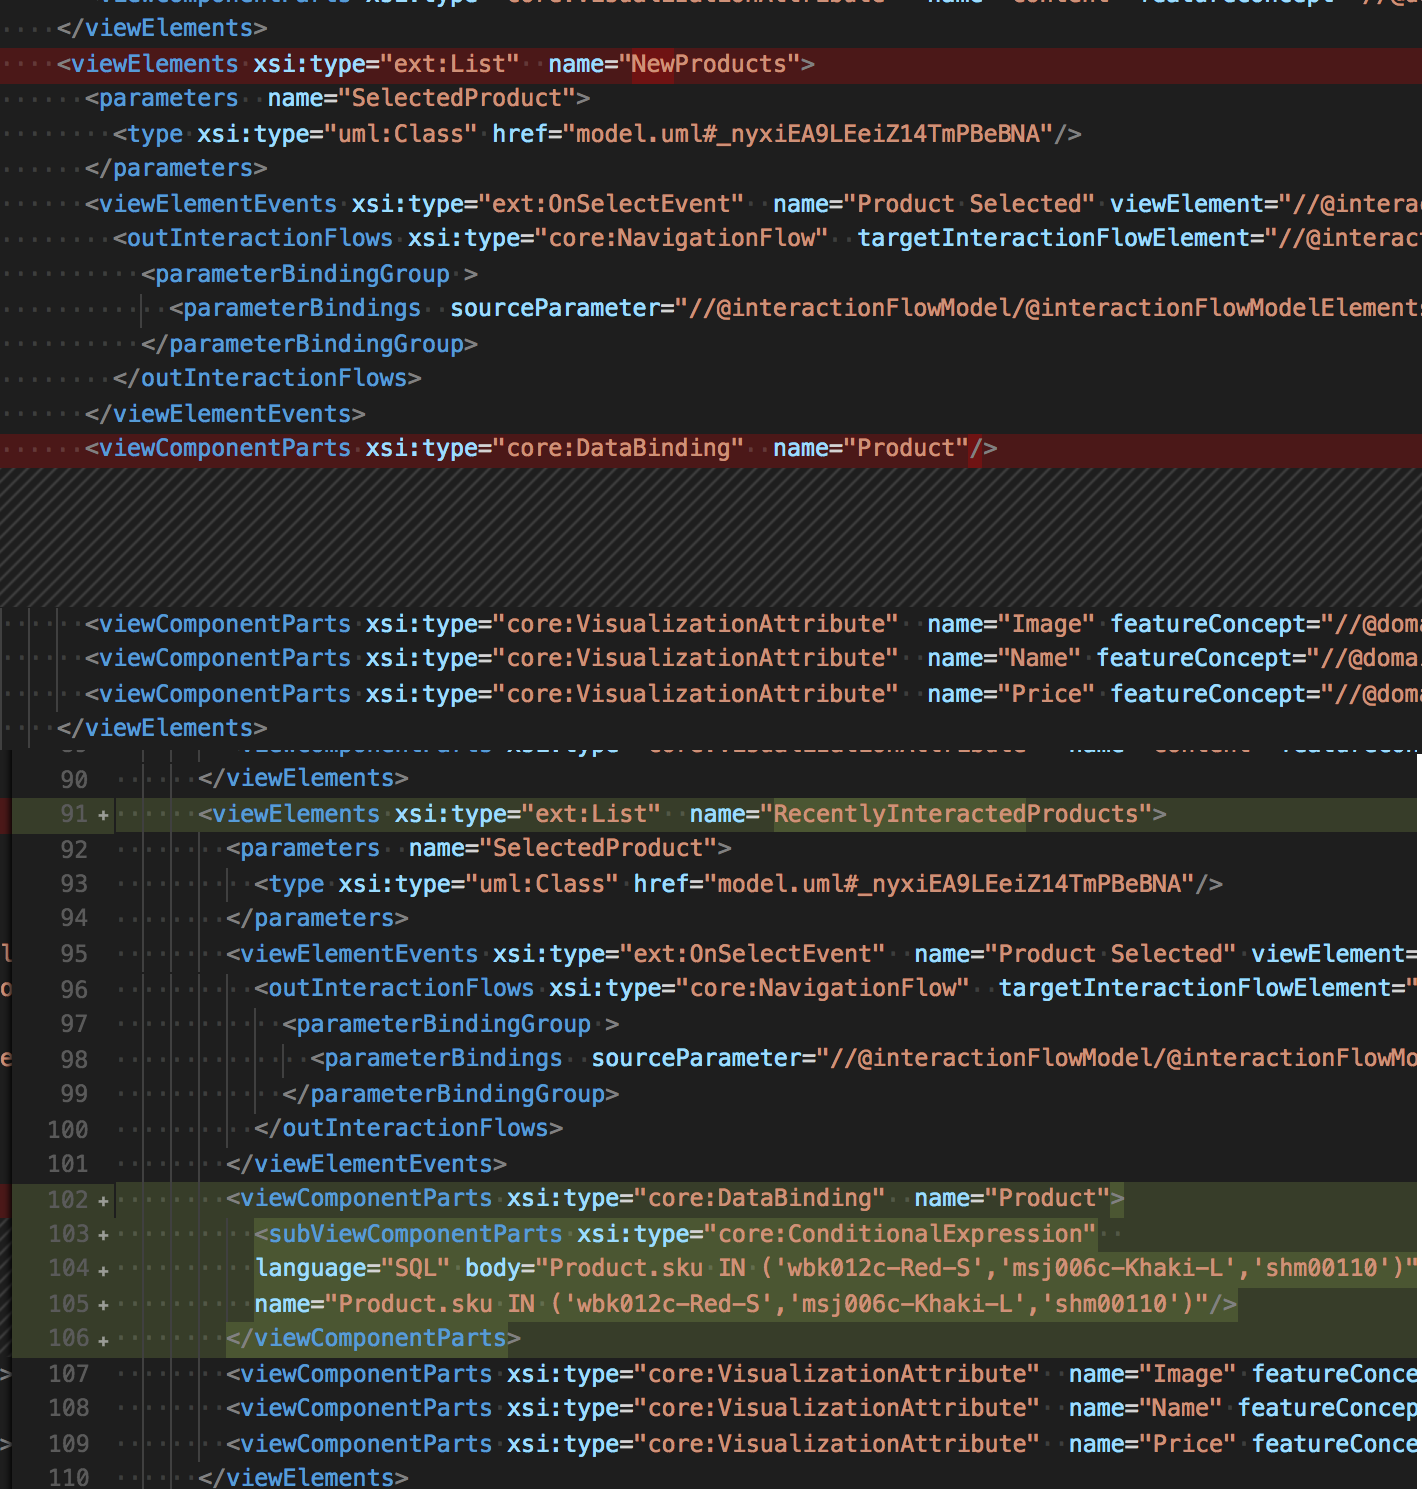
\includegraphics[height=12cm]{images/madison/ifm-homepage-transformation.png}
  \caption{IFML Homepage transformation example}
  \label{fig:ifml-transformation-example}
\end{figure}
\vspace{0.5cm}

\subsection{Header}
\label{header-updates}

Leveraging once more the \textit{RealUsageData:ActionData}, the Header node of the \textit{IFMLModel} describing the top area in the Madison Island website could also be enhanced to show a list of recent actions performed by customers in the physical stores that generated reward points.  This can be achieved by appending an instance of \textit{List View Component} to the \textit{interactionFlowModelElements} parent node, called \textit{RecentRewardActions}. This instance is then linked to the Rewards \textit{Data Binding} entity, which allows the visualization of the \textit{Action Name} and \textit{Points Attribution} properties to the front-end, as shown in the following snippet of \textit{IFMLModel} code:

\vspace{0.5cm}
\lstset{language=XML}
\begin{lstlisting} 
  <interactionFlowModelElements xsi:type="ext:IFMLWindow"  name="Header" isLandmark="true">
  <viewElements xsi:type="ext:List"  name="NavigationMenu">
   ...
  </viewElements>
  <viewElements xsi:type="ext:Form"  name="SearchForm">
   ...
  </viewElements>
  <viewElements xsi:type="core:ViewComponent"  name="TopLinks"/>
  <viewElements xsi:type="core:ViewComponent"  name="LanguageSwitch"/>

  <!-- ADDED NODE -->
  <viewElements xsi:type="ext:List"  name="RecentRewardActions">
    <viewComponentParts xsi:type="core:DataBinding"  name="Rewards" domainConcept="//@domainModel/@domainElements.13"/>
    <viewComponentParts xsi:type="core:VisualizationAttribute"  name="Action Name" featureConcept="//@domainModel/@domainElements.15"/>
    <viewComponentParts xsi:type="core:VisualizationAttribute"  name="Points Attribution" featureConcept="//@domainModel/@domainElements.14"/>
  </viewElements>
  <!-- ADDED NODE -->

  </interactionFlowModelElements>
\end{lstlisting}
\vspace{0.5cm}

\subsection{Category Page}
\label{category-page-updates}

In light of the information gathered in the Real Usage Data model about the recently viewed products available in the \textit{RealUsageData:WebData} node, the Category page can be enhanced by appending an additional visual element to the user interface for tracking that information.

To do so, we filter out the RealUsageData model, fetching the nodes containing a \textit{parameterBindingGroup} property and including a Product reference like the following entries:

\vspace{0.5cm}
\lstset{language=XML}
\begin{lstlisting} 
      <data xsi:type="RealUsageData:WebData"
      ID="3"
      name="AccessLog"
      userID="3045678"
      date="2017-11-29T07:08:40.000+0100"
      viewContainer="Category #15"
      viewComponent="ProductList"
      eventType="click"
      parameterBindingGroup="Product/404"
      logEntry="GET /men/shirts/plaid-cotton-shirt-476.html 200 0 - 29505"/>
      
      <data xsi:type="RealUsageData:WebData"
      ID="4"
      name="AccessLog"
      userID="3045678"
      date="2017-12-04T06:37:15.000+0100"
      viewContainer="Product #404"
      viewComponent="RelatedProductList"
      eventType="click"
      parameterBindingGroup="Product/413"
      logEntry="GET /core-striped-sport-shirt-551.html 200 0 - 29505"/>

      <data xsi:type="RealUsageData:WebData"
      ID="8"
      name="AccessLog"
      userID="3045678"
      date="2017-12-04T06:38:20.000+0100"
      viewContainer="Search Results"
      viewComponent="ProductList"
      eventType="click"
      parameterBindingGroup="Product/407"
      logEntry="GET /stretch-cotton-blazer-587.html 200 0 - 29505"/>
\end{lstlisting}
\vspace{0.5cm}

With the data described above, we can then proceed with transforming the initial \textit{IFMLModel} for the Category page, appending to it a \textit{RecentlyViewedProducts} section in the form of a \textit{List View Component} bound to the Product \textit{Data Binding} entity.

This new IFML item would be responsible for presenting customers with the thumbnails, names, and prices of these products, separating them through a distinct \textit{ConditionalExpression}. That expression maps the children node of the \textit{RealUsageData:WebData} dataset shown previously, before finally returning the items in the order they were browsed, and regardless of the display mode property of the Category itself (Figure \ref{fig:recently-viewed-ifml-definition}).

\vspace{0.5cm}
\begin{figure}[H]
  \centering
    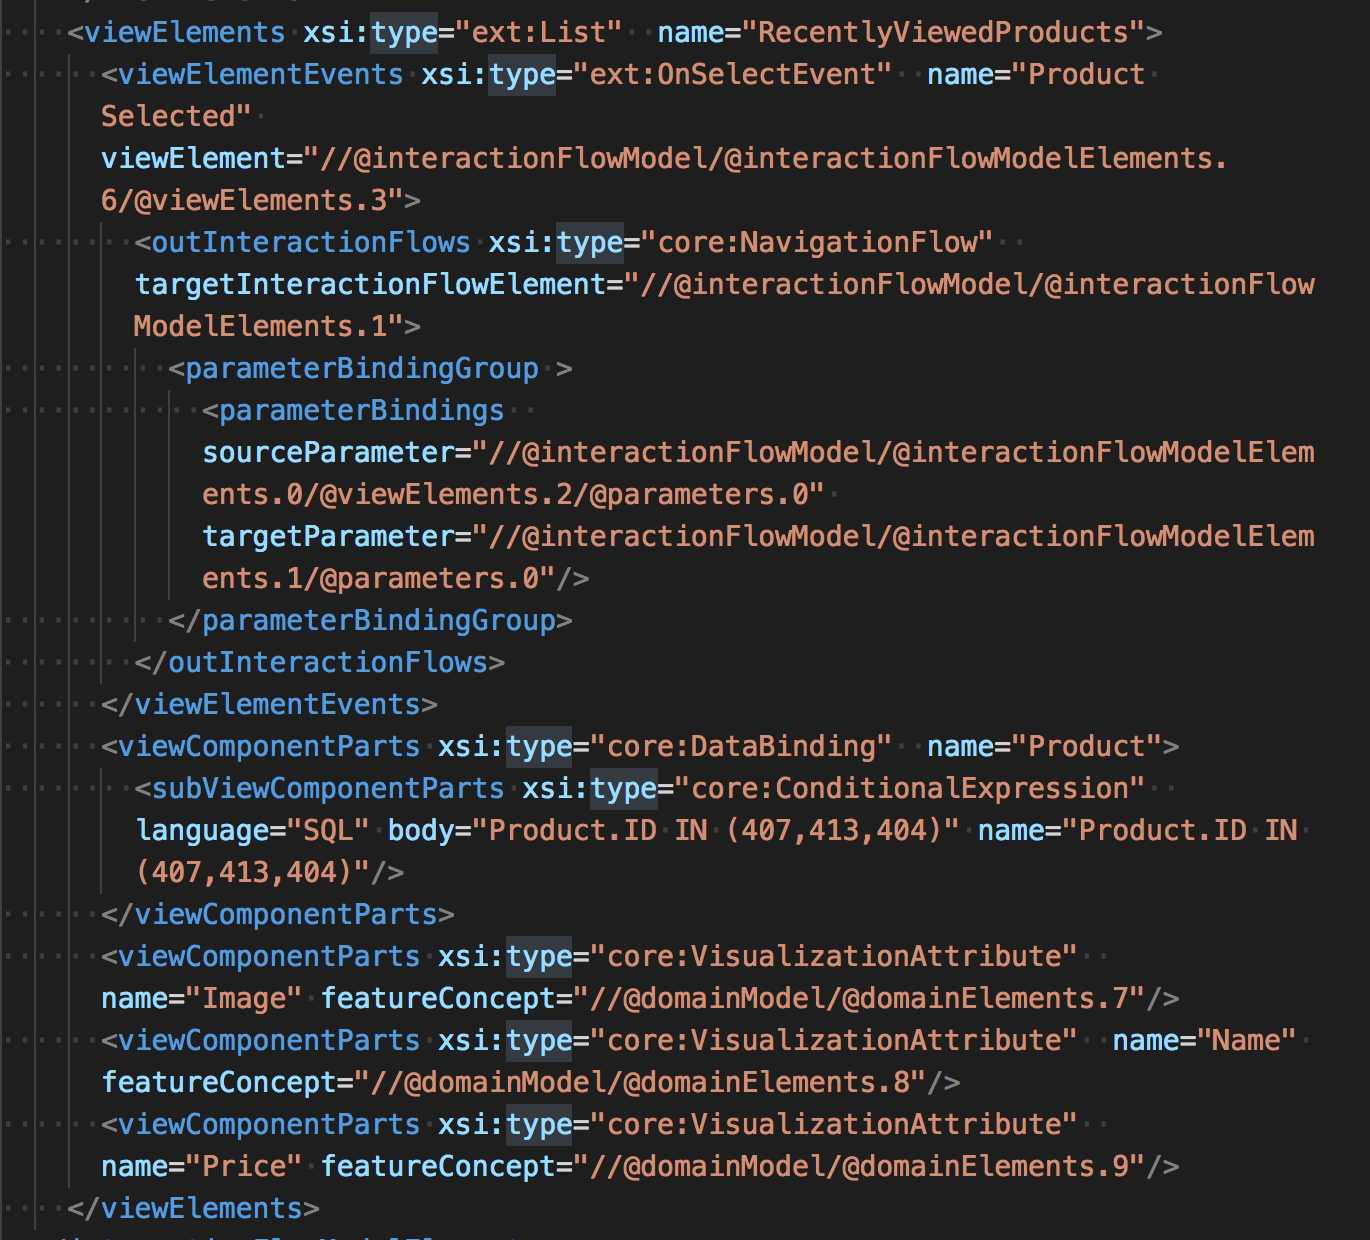
\includegraphics[height=12cm]{images/madison/ifml-recently-viewed.png}
  \caption{Recently Viewed IFML definition snippet}
  \label{fig:recently-viewed-ifml-definition}
\end{figure}
\vspace{0.5cm}

\subsection{Product Page}
\label{product-page-updates}

As far as the possible improvements on the product page of the Madison Island website are concerned, we concentrated on the Related Products widget shown below the Add To Cart section. In the first \textit{IFMLModel}, the list of products related to the currently shown item has no particular assigned logic. Our potential transformation is to extend the \textit{viewElements} node of the \textit{IFMLModel}, taking into account users browsing patterns that have been identified by examining the RealUsageData instances entries.

For example, we could have discovered that, during a same recorded sessions, the \textbf{Core Striped Sport Shirt} and the \textbf{Plaid Cotton Shirt} product pages are frequently browsed together. That could be done by analysing the values set in the \textit{viewContainer}, \textit{viewComponent}, and \textit{parameterBindingGroup} properties for the nodes belonging to the \textit{RealUsageData:WebData} dataset. Such change allows us to take advantage of this correlation, pushing specific products on the Related Products section and consequently offering a more tailored user experience.

The change on the starting \textit{IFMLModel} that would occur in that case restricts the \textit{Data Binding} scope, appending a \textit{subViewComponentParts} to it. That change limits the products collection to the computed set of related products SKUs. The additional \textit{ConditionalExpression} would also be bound to a specific \textit{ActivationExpression}, which would enable the above mentioned filtering only when a customised collection is available for the current product. 

From a \textit{IFMLModel} code perspective, we would transition from the following node configuration for the \textit{List View Component} that controls the Related Product widget:

\vspace{0.5cm}
\lstset{language=XML}
\begin{lstlisting} 
  <viewElements xsi:type="ext:List"  name="RelatedProductList">
  <viewElementEvents xsi:type="ext:OnSelectEvent"  name="Product Selected" viewElement="//@interactionFlowModel/@interactionFlowModelElements.1/@viewElements.2">
    ...
  </viewElementEvents>
  <viewComponentParts xsi:type="core:DataBinding"  name="Product"/>
  <viewComponentParts xsi:type="core:VisualizationAttribute"  name="Image" featureConcept="//@domainModel/@domainElements.7"/>
  <viewComponentParts xsi:type="core:VisualizationAttribute"  name="Name" featureConcept="//@domainModel/@domainElements.8"/>
  <viewComponentParts xsi:type="core:VisualizationAttribute"  name="Price" featureConcept="//@domainModel/@domainElements.9"/>
</viewElements>
\end{lstlisting}
\vspace{0.5cm}

to this one:

\vspace{0.5cm}
\lstset{language=XML}
\begin{lstlisting} 
  <viewElements xsi:type="ext:List"  name="RelatedProductList">
  <viewElementEvents xsi:type="ext:OnSelectEvent"  name="Product Selected" viewElement="//@interactionFlowModel/@interactionFlowModelElements.1/@viewElements.2">
      ...
  </viewElementEvents>
  <viewComponentParts xsi:type="core:DataBinding"  name="Product">
    <subViewComponentParts xsi:type="core:ConditionalExpression"  language="SQL" body="Product.ID IN getCustomizedRelatedProducts()" name="Product.ID IN getCustomizedRelatedProducts" activationExpression="//@interactionFlowModel/@interactionFlowModelElements.17"/>
  </viewComponentParts>
  <viewComponentParts xsi:type="core:VisualizationAttribute"  name="Image" featureConcept="//@domainModel/@domainElements.7"/>
  <viewComponentParts xsi:type="core:VisualizationAttribute"  name="Name" featureConcept="//@domainModel/@domainElements.8"/>
  <viewComponentParts xsi:type="core:VisualizationAttribute"  name="Price" featureConcept="//@domainModel/@domainElements.9"/>
</viewElements>
\end{lstlisting}
\vspace{0.5cm}

Moreover, the \textit{ActivationExpression} defined by the \textit{interactionFlowModelElements} XPath expression presented above links to a node responsible for controlling the feature with the following content:

\vspace{0.5cm}
\lstset{language=XML}
\begin{lstlisting} 
<interactionFlowModelElements 
  xsi:type="core:ActivationExpression" id="CurrentProduct.hasCustomizedRelatedProduct" language="SQL" body="CurrentProduct.hasCustomizedRelatedProduct()">
</interactionFlowModelElements>

\end{lstlisting}
\vspace{0.5cm}
\subsection{Shopping Cart}
\label{shopping-cart-updates}

As described in \ref{shopping-cart-page-overview}, the Shopping Cart page model includes two main sections. The first is a \textit{List Product List} component, responsible for the interactions with the cart items. The second is the \textit{IFMLWindow}, used for grouping the actions triggered by customers when they apply discounts or estimate shipping and taxes for their current quote.

\vspace{0.5cm}
\begin{figure}[H]
  \centering
    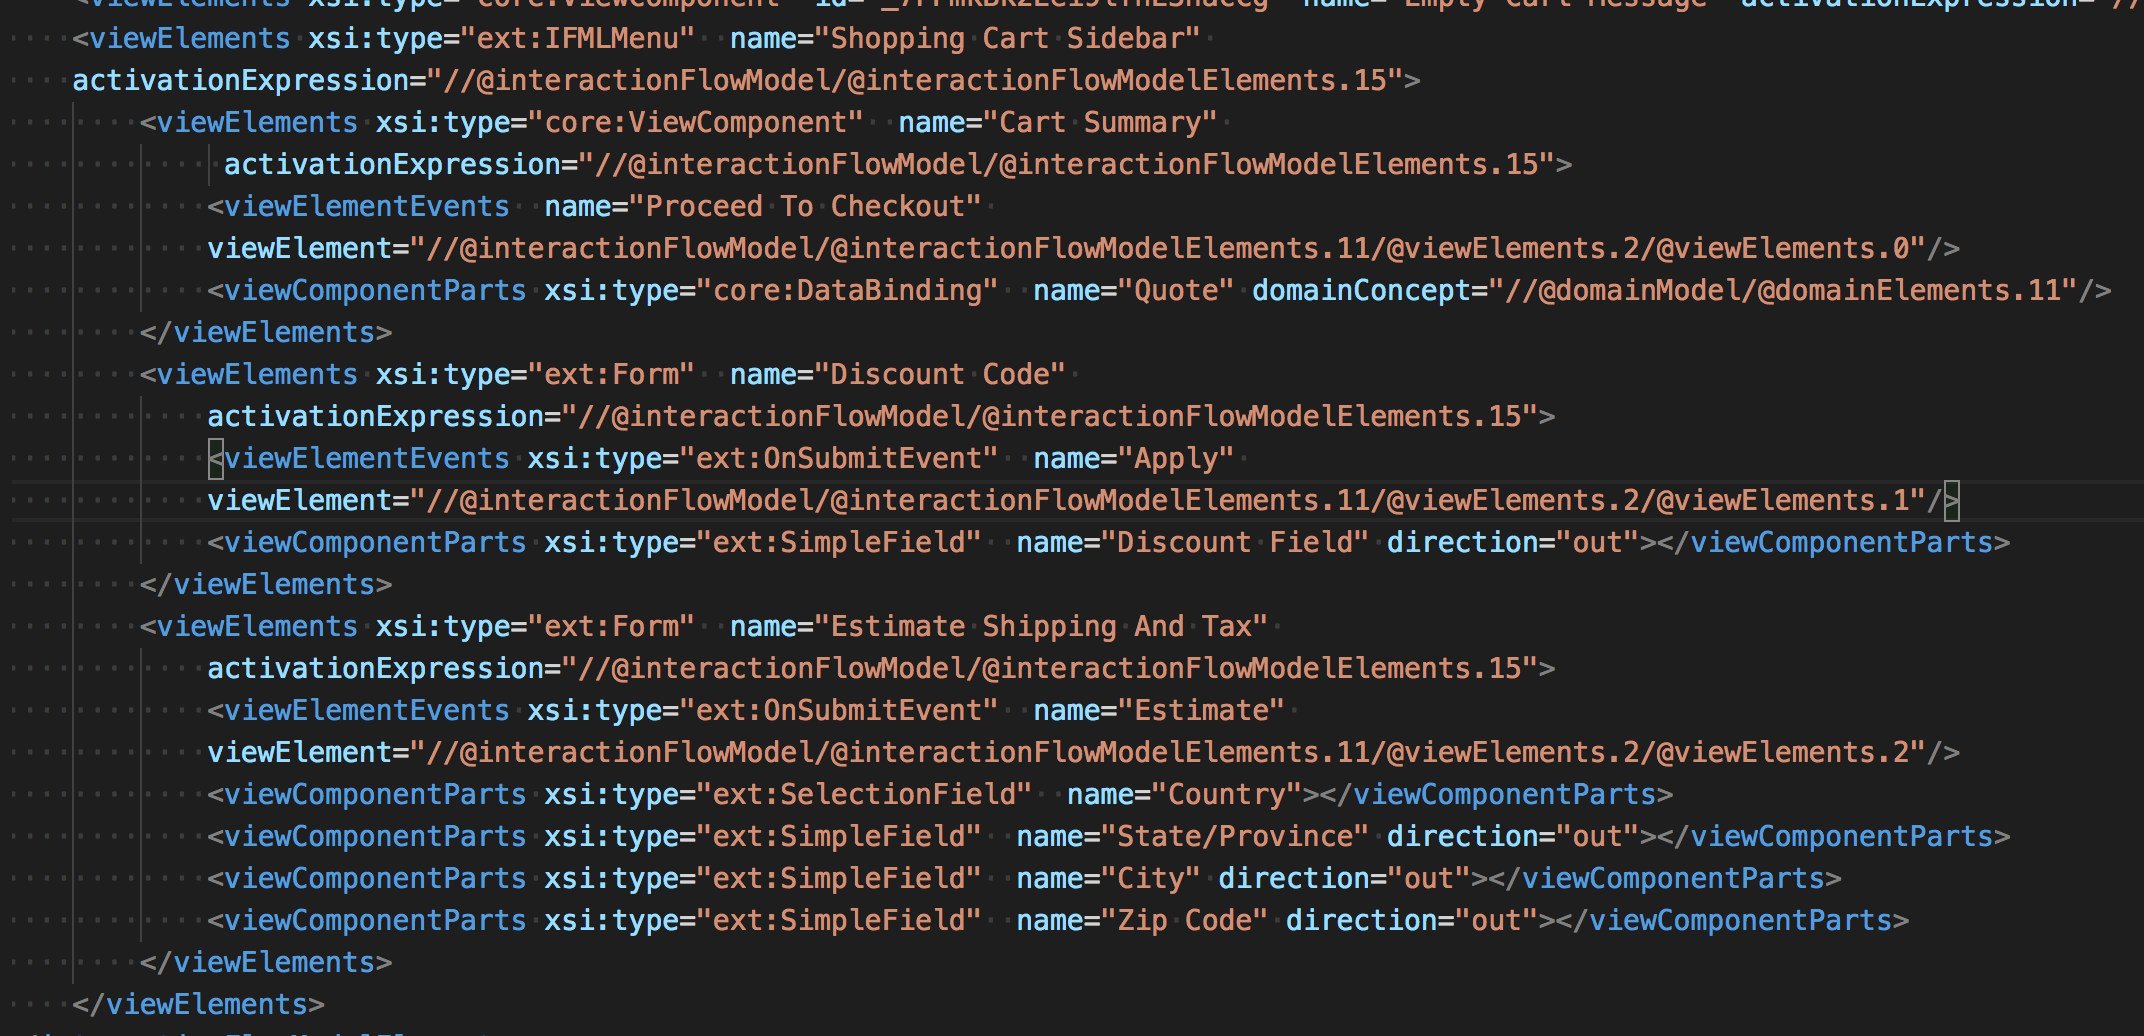
\includegraphics[width=12cm]{images/madison/ifml-shopping-cart-sidebar.png}
  \caption{Shopping Cart Sidebar IFML definition snippet}
  \label{fig:shopping-cart-sidebar-ifml-definition}
\end{figure}
\vspace{0.5cm}

Along with the cases analysed previously and by applying the data from the Real Data Usage model, we can modify and extend the interaction flow of this page by adding a new \textit{View Component}. That component shows the Reward points accumulated by the user in the Shopping Cart Sidebar (Figure \ref{fig:shopping-cart-sidebar-ifml-definition}). The component not only displays the information by the \textit{Data Binding} with the Reward entity, but also controls the \textit{Event} associated with the \textbf{``Apply Discount"} button and the \textit{Action} connected to it. 
The structure of this new node, which gets appended to its parent \textit{IFMLMenu}, is as follows:

\vspace{0.5cm}
\lstset{language=XML}
\begin{lstlisting} 
  <viewElements xsi:type="core:ViewComponent" name="Applicable Reward Points">
    <viewElementEvents xsi:type="ext:OnSelectEvent" name="Apply Reward Points" viewElement="//@interactionFlowModel/@interactionFlowModelElements.11/@viewElements.2/@viewElements.3">
        <outInteractionFlows xsi:type="core:NavigationFlow" targetInteractionFlowElement="//@interactionFlowModel/@interactionFlowModelElements.18/@actionEvents.0"/>
    </viewElementEvents>
    <viewComponentParts xsi:type="core:DataBinding" name="Reward"/>
    <viewComponentParts xsi:type="core:VisualizationAttribute"  name="Available Reward Points" featureConcept="//@domainModel/@domainElements.14"/>
</viewElements>
\end{lstlisting}
\vspace{0.5cm}

\newpage
\section{Updated web models}

In this section, we present an overview of the updated IFMLModels for the Madison Island website based on the transformations discussed in the last chapter. We also describe how their IFMLDiagrams and corresponding website front-end screens would look like.

\subsection{Homepage}

According to what we described in \ref{homepage-updates}, the enhanced homepage presented to the customer would show a custom banner carousel and a product widget, both containing items and categories with which the user interacted in the retail store.

\vspace{0.5cm}
\begin{figure}[H]
  \centering
    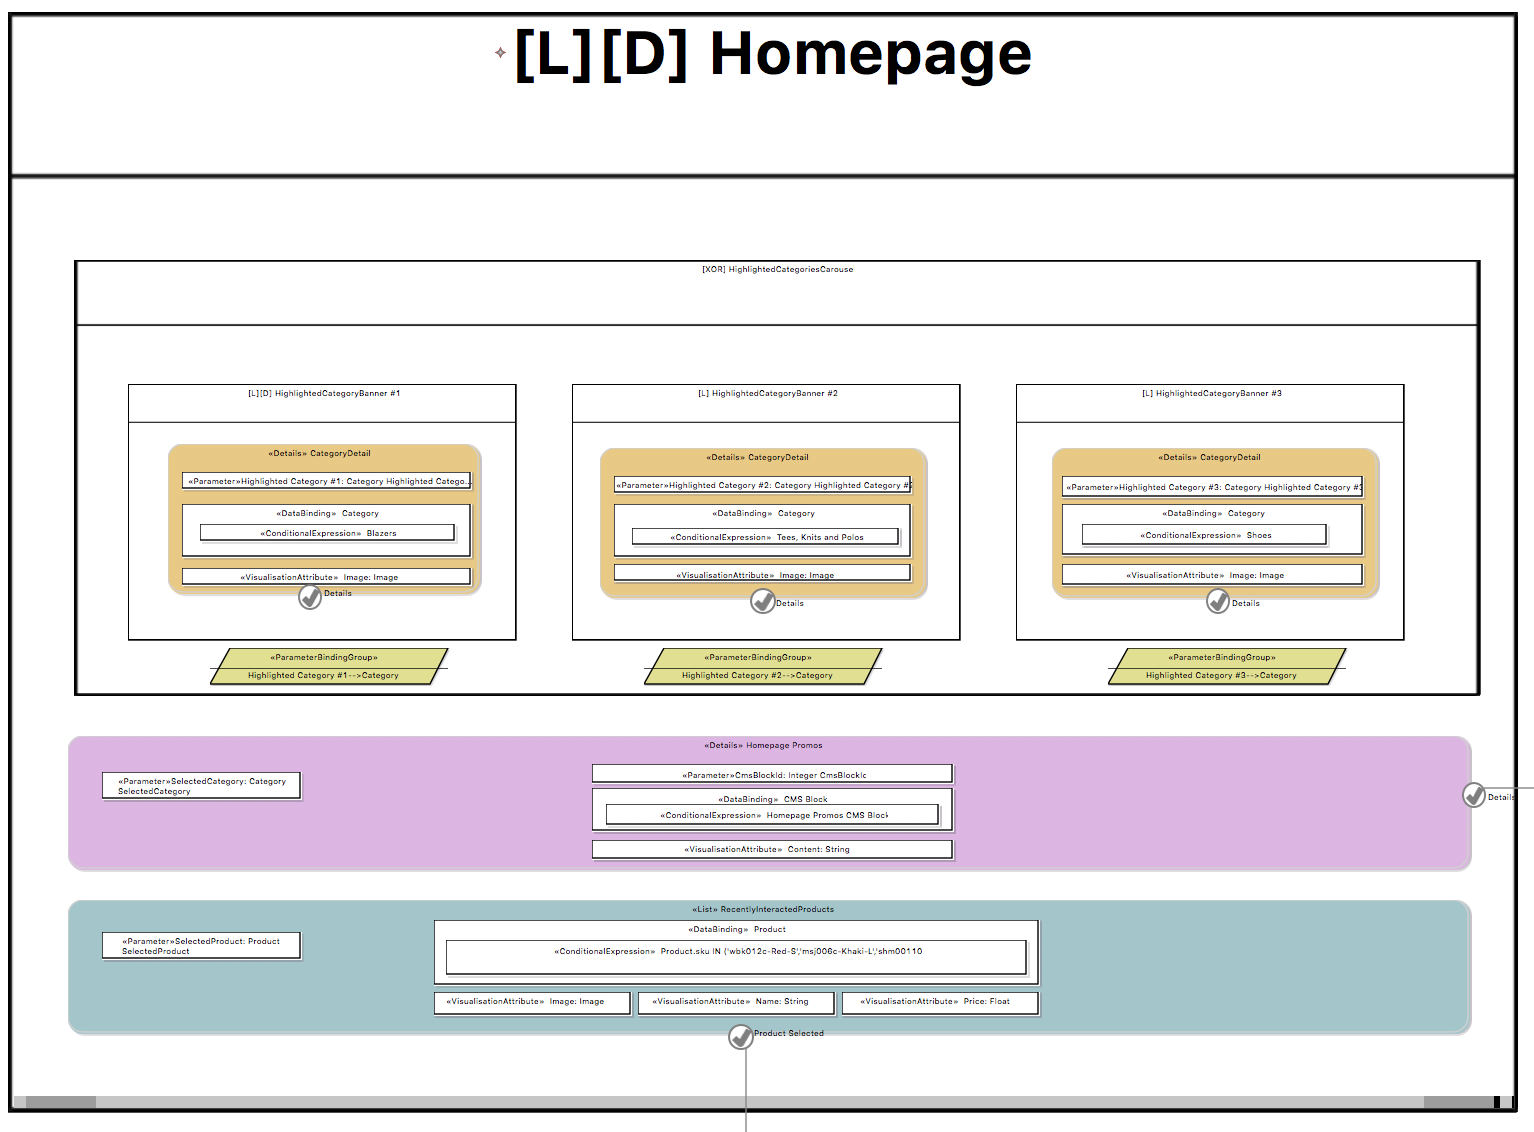
\includegraphics[height=9cm]{images/diagrams/after/ifml-homepage.png}
  \caption{Updated Homepage IFML Diagram}
  \label{fig:ifml-after-homepage}
\end{figure}

\begin{figure}[H]
  \centering
    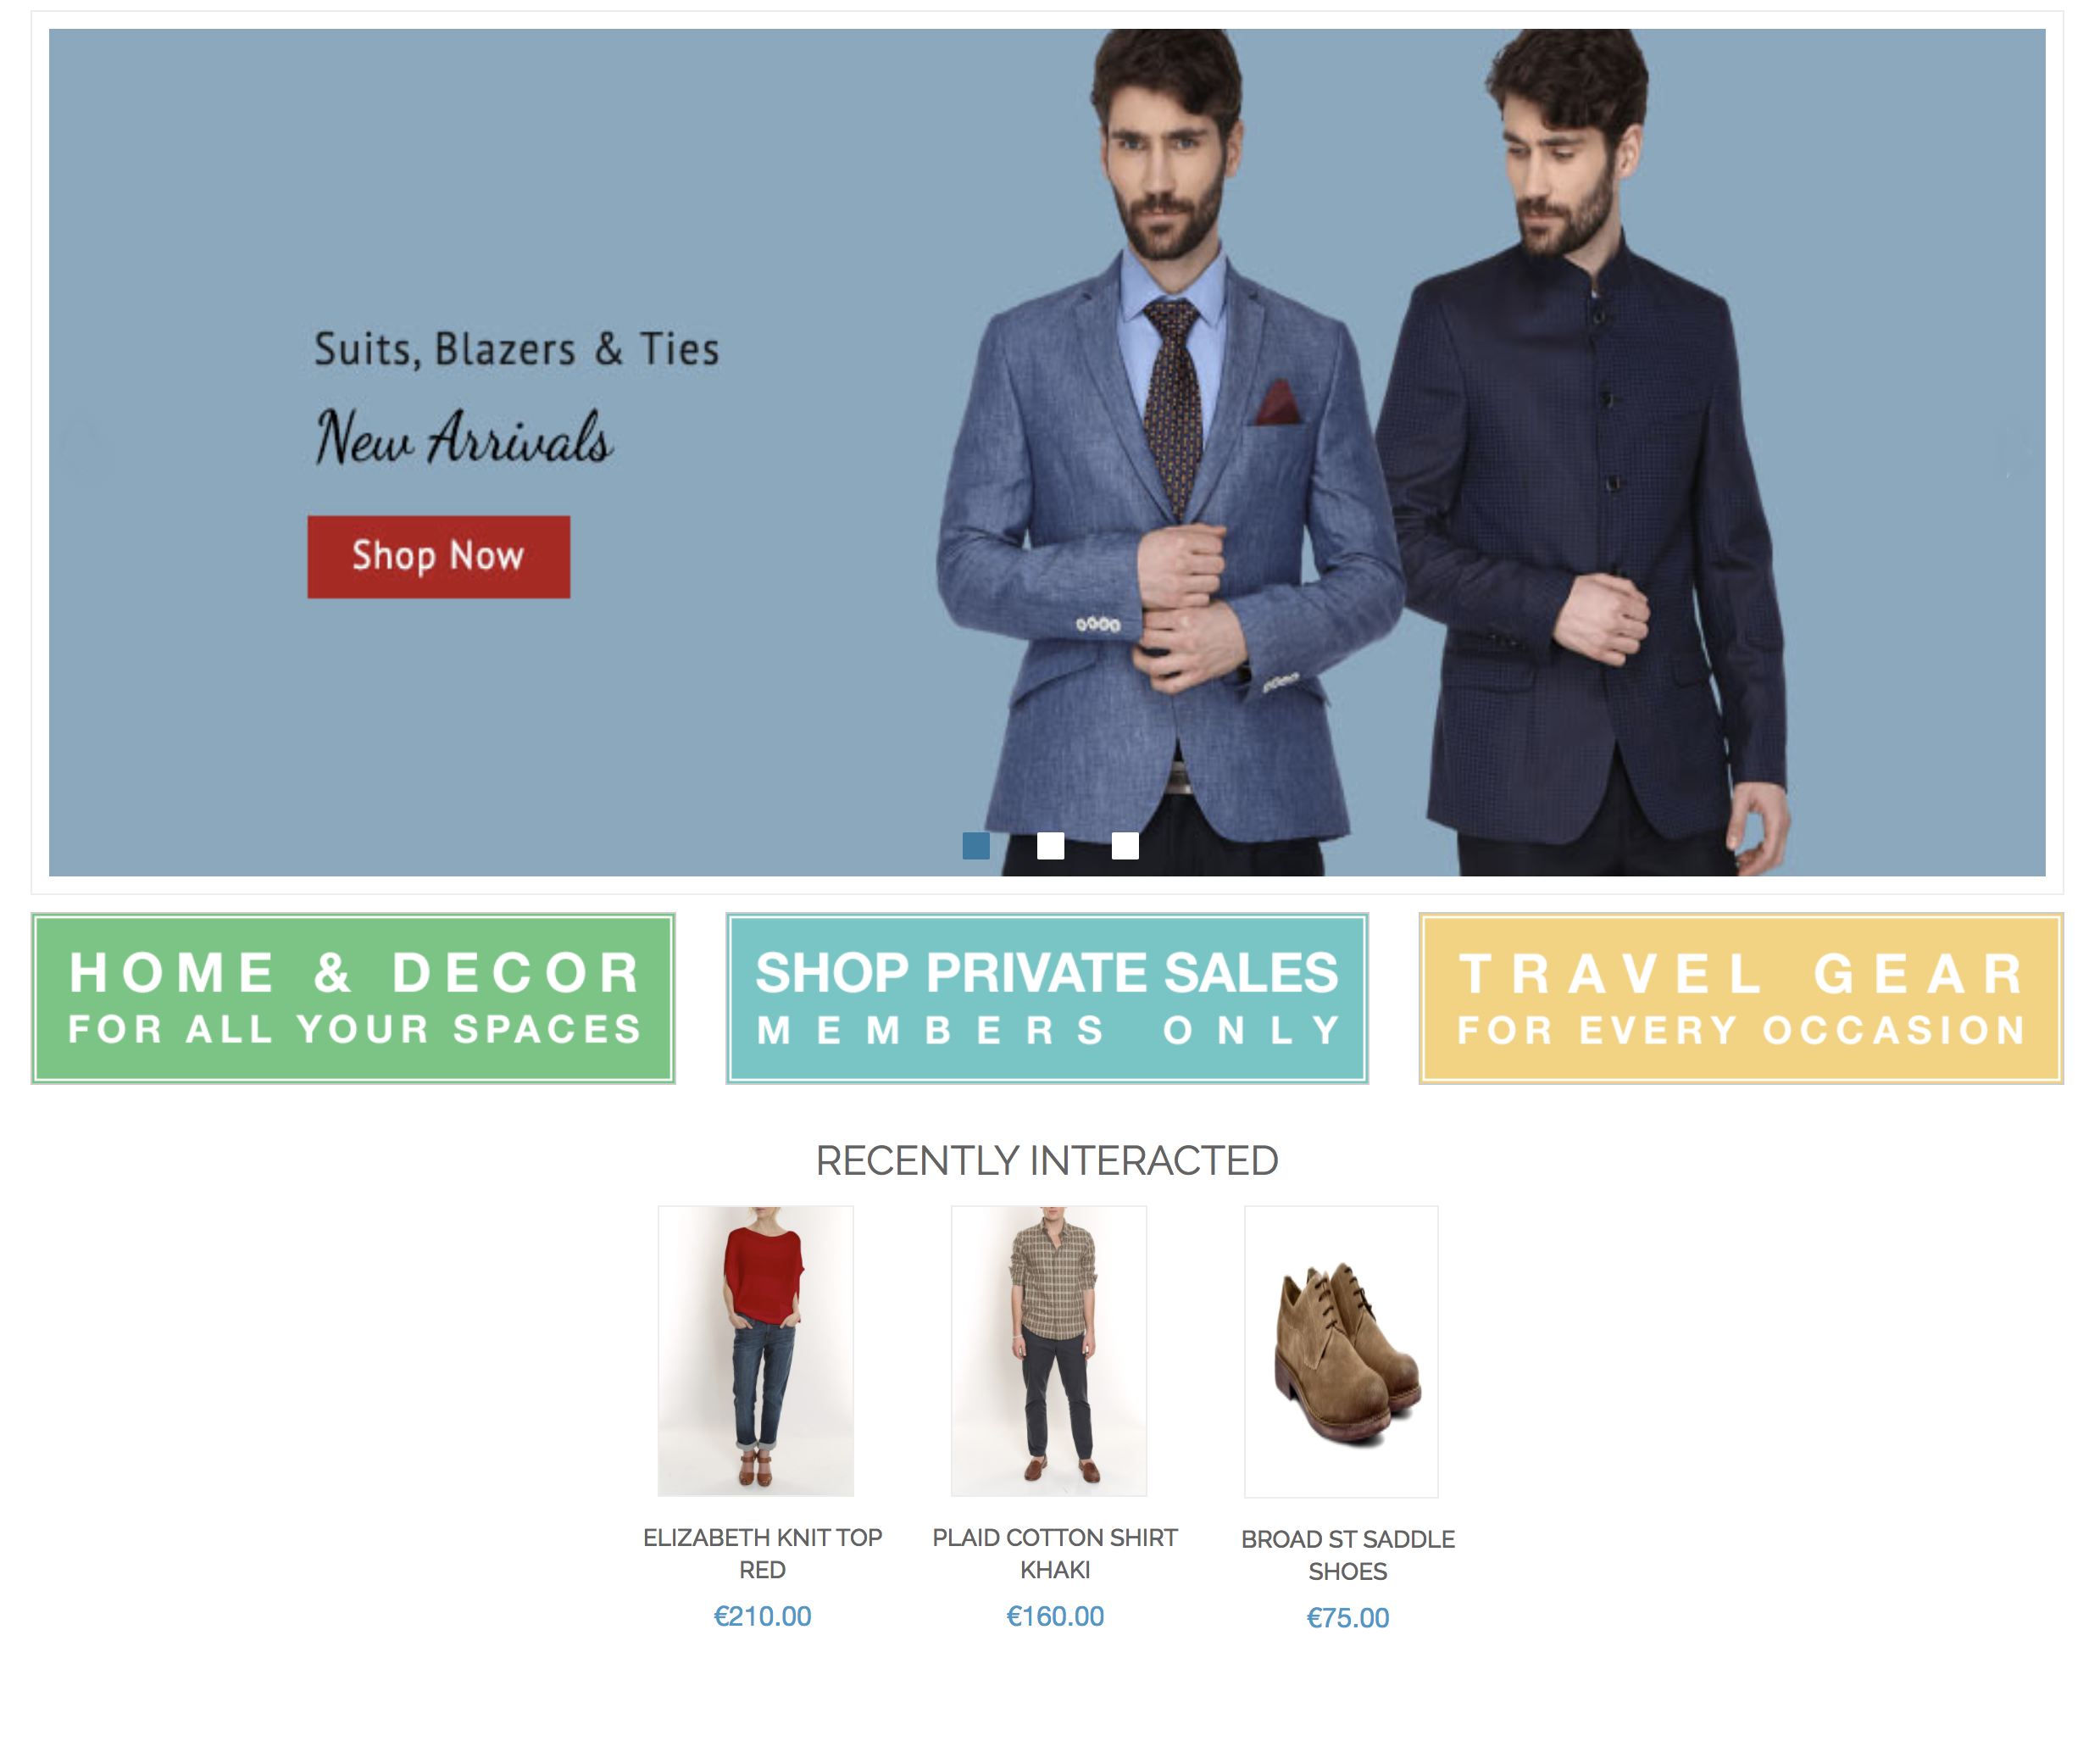
\includegraphics[height=9cm]{images/diagrams/after/desktop-homepage.png}
  \caption{Updated Homepage Desktop}
  \label{fig:desktop-after-homepage}
\end{figure}
\vspace{0.5cm}

\newpage
\subsection{Header}

After transforming its IFMLModel component (\ref{header-updates}), the shared header section on the website reveals new information through a new widget. This widget is aligned on the right side of the area used for advertising the actions taken by the user in the retail store and their respective rewarded points.

\vspace{0.5cm}
\begin{figure}[H]
  \centering
    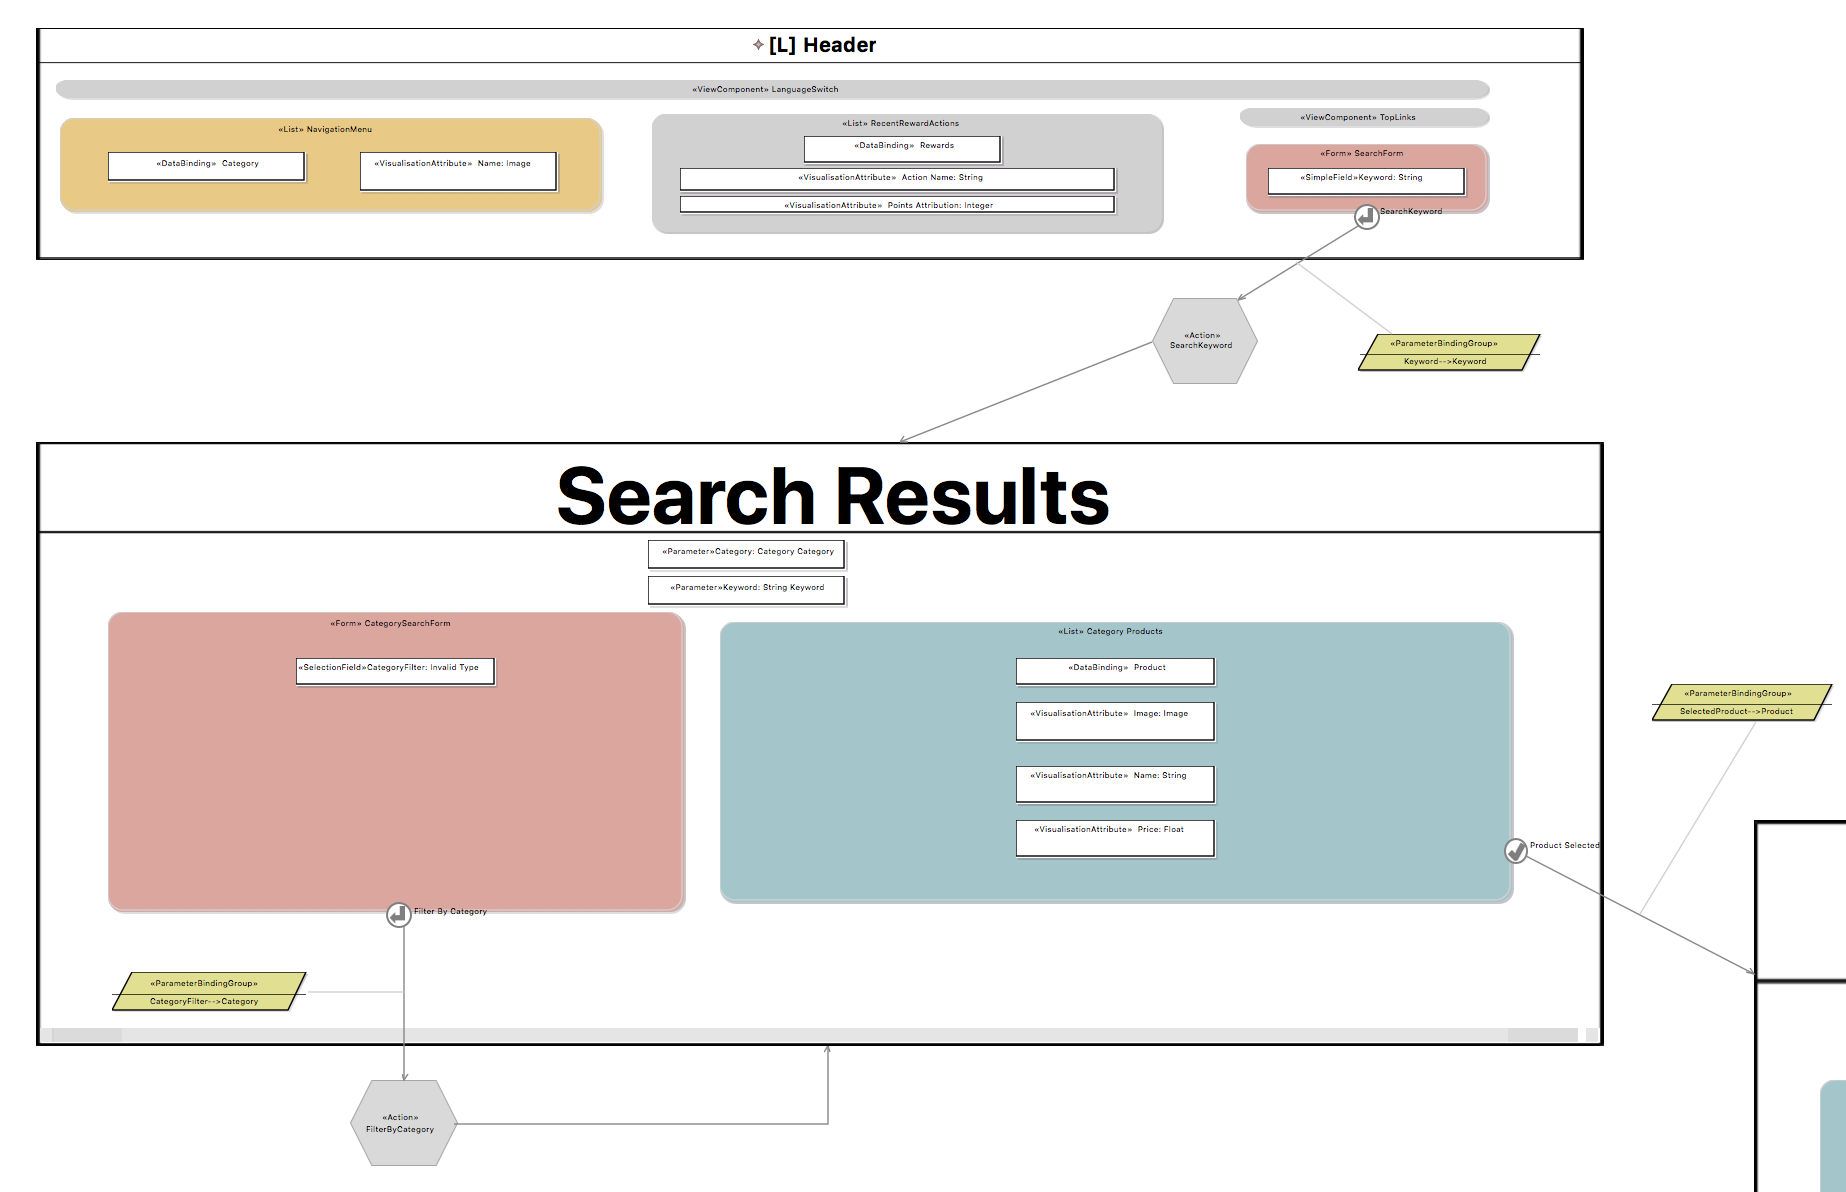
\includegraphics[width=14cm]{images/diagrams/after/ifml-header.png}
  \caption{Updated Header IFML Diagram}
  \label{fig:ifml-after-header}
\end{figure}

\begin{figure}[H]
  \centering
    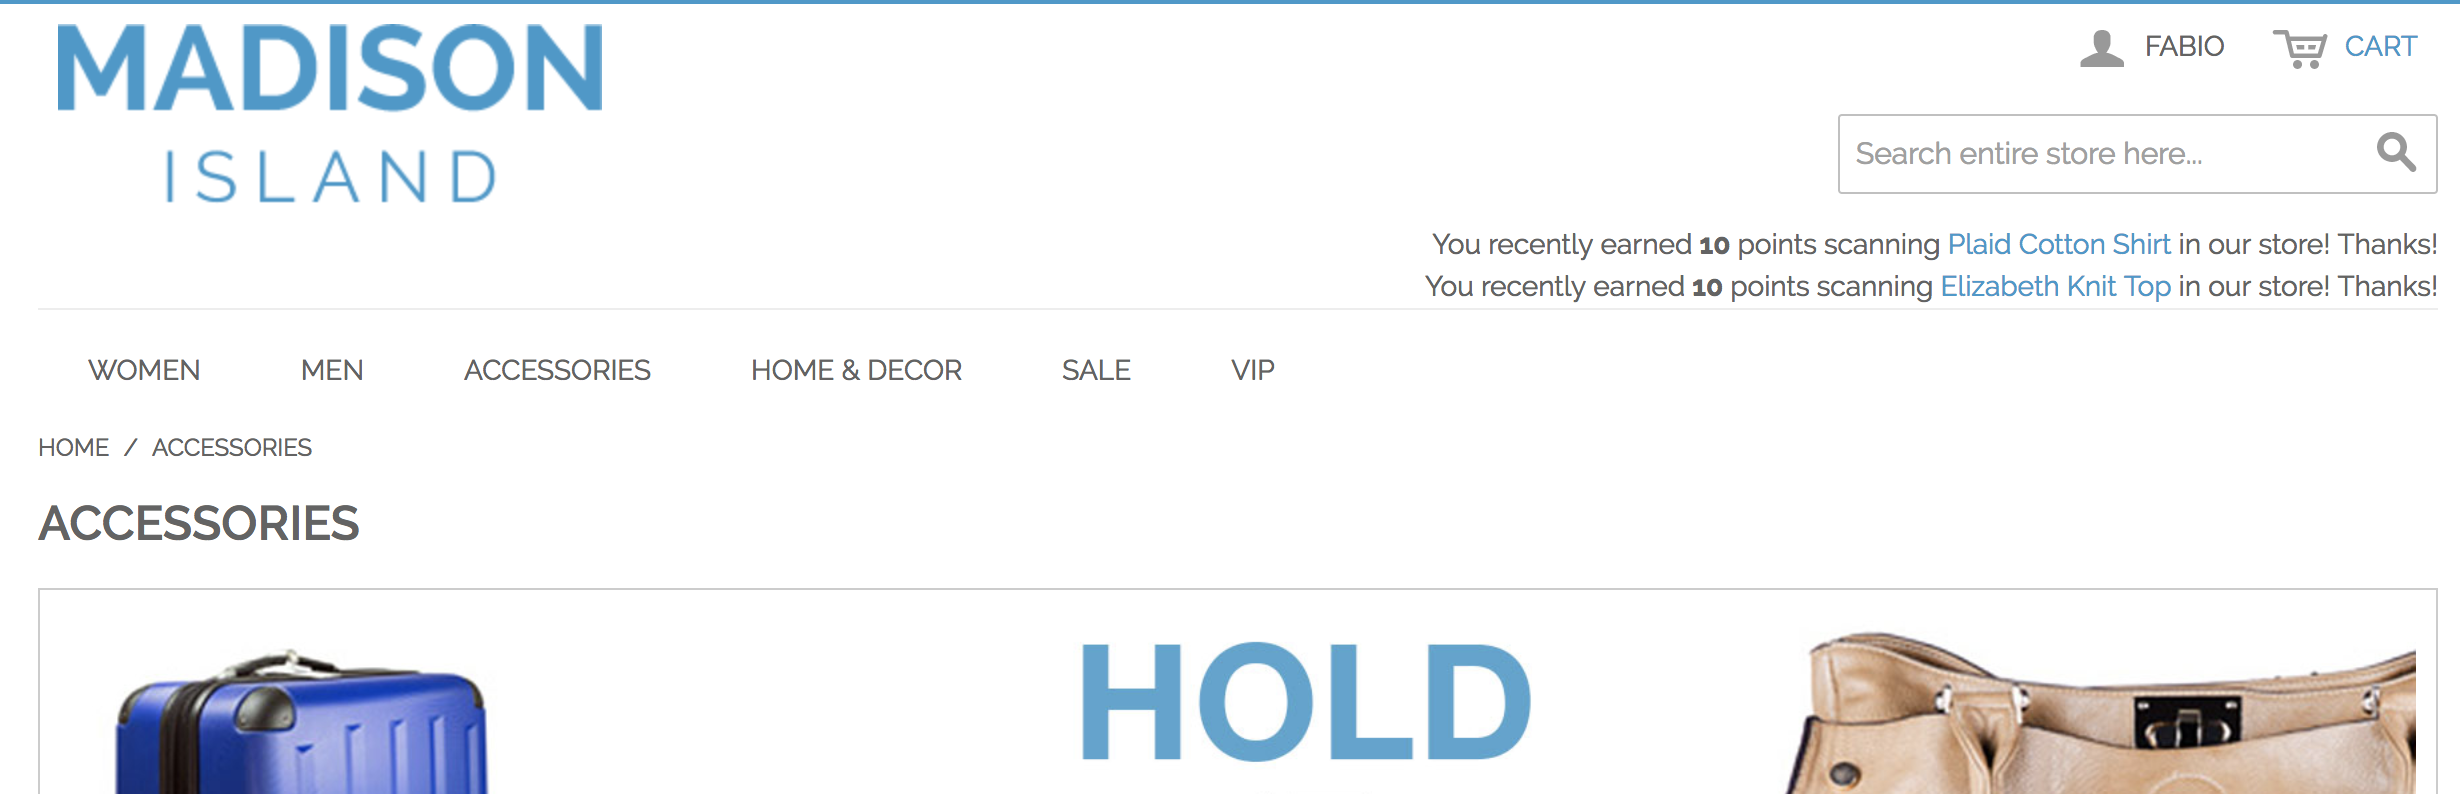
\includegraphics[width=14cm]{images/diagrams/after/desktop-header.png}
  \caption{Updated Header Desktop Version}
  \label{fig:desktop-after-header}
\end{figure}
\vspace{0.5cm}

\newpage
\subsection{Category Page}

Regardless of the DisplayMode property set for each Category Page on the eCommerce platform, the updated web model presents a vertical section on the right sidebar. That section maps the URLs browsed recently in a same user session that have been identified during the model transformation phase (\ref{category-page-updates}).

\vspace{0.5cm}
\begin{figure}[H]
  \centering
    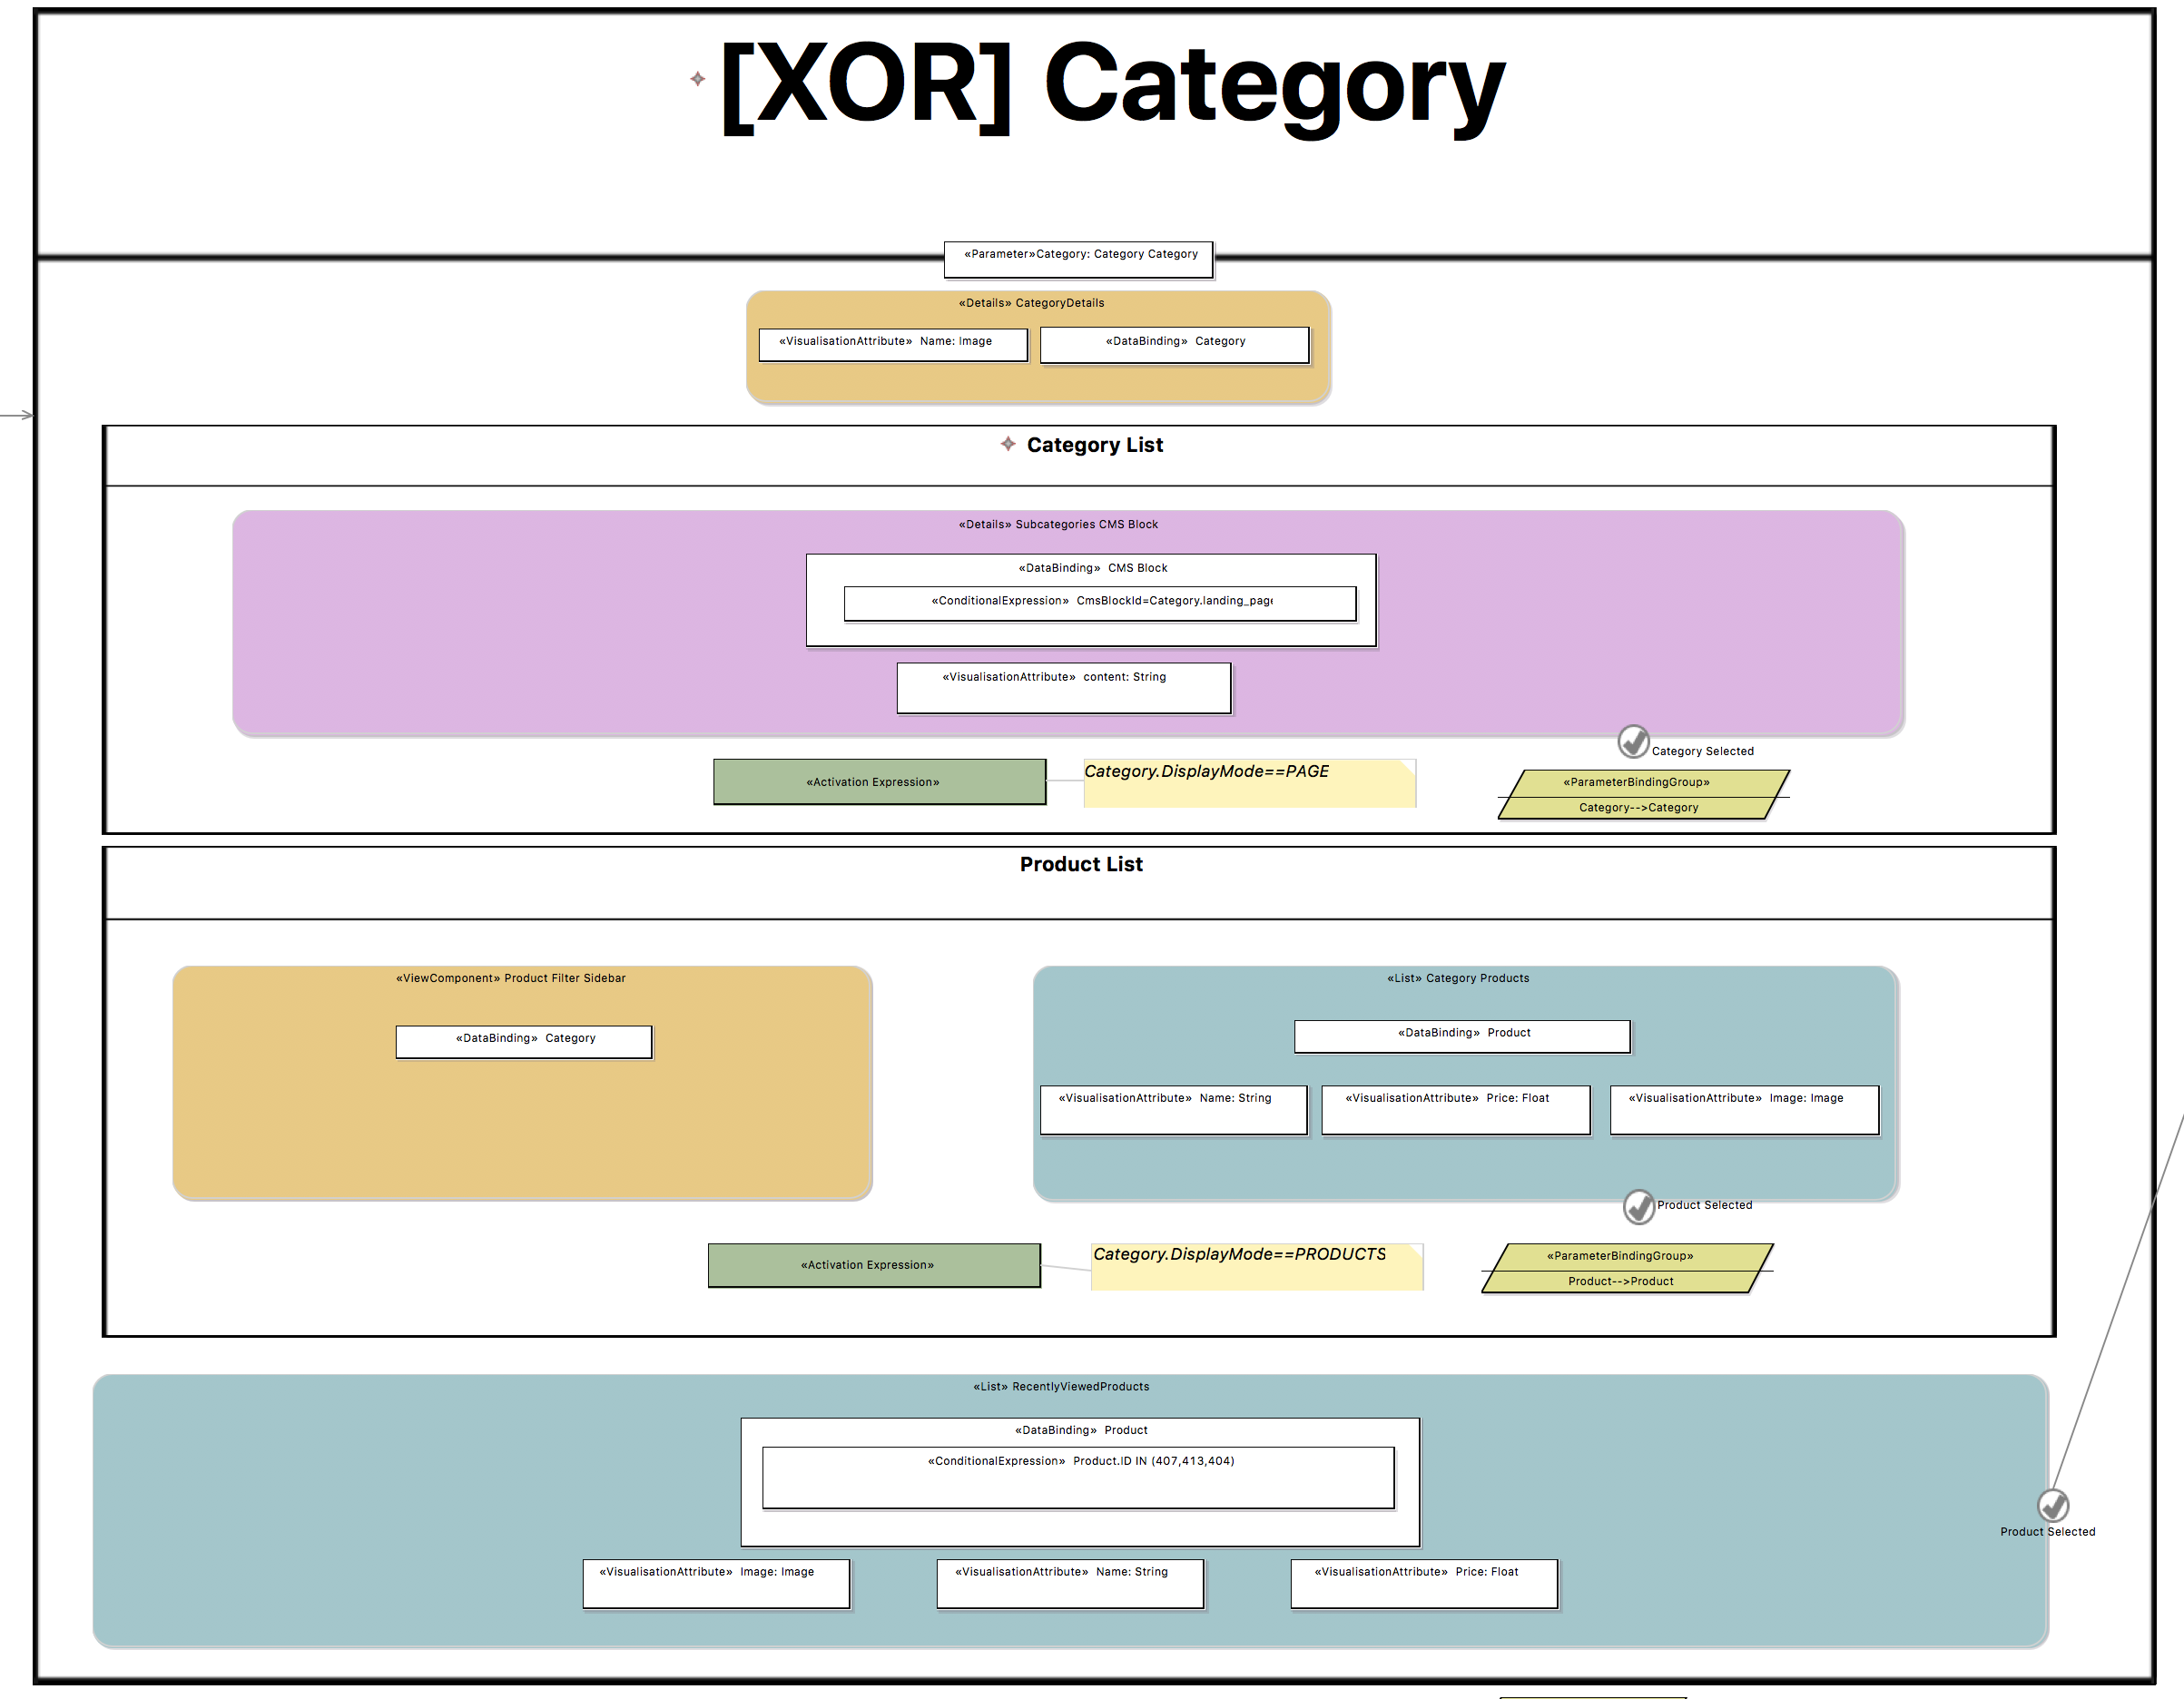
\includegraphics[height=12cm]{images/diagrams/after/ifml-category.png}
  \caption{Updated Category Page IFML Diagram}
  \label{fig:ifml-after-category}
\end{figure}

\begin{figure}[H]
  \centering
    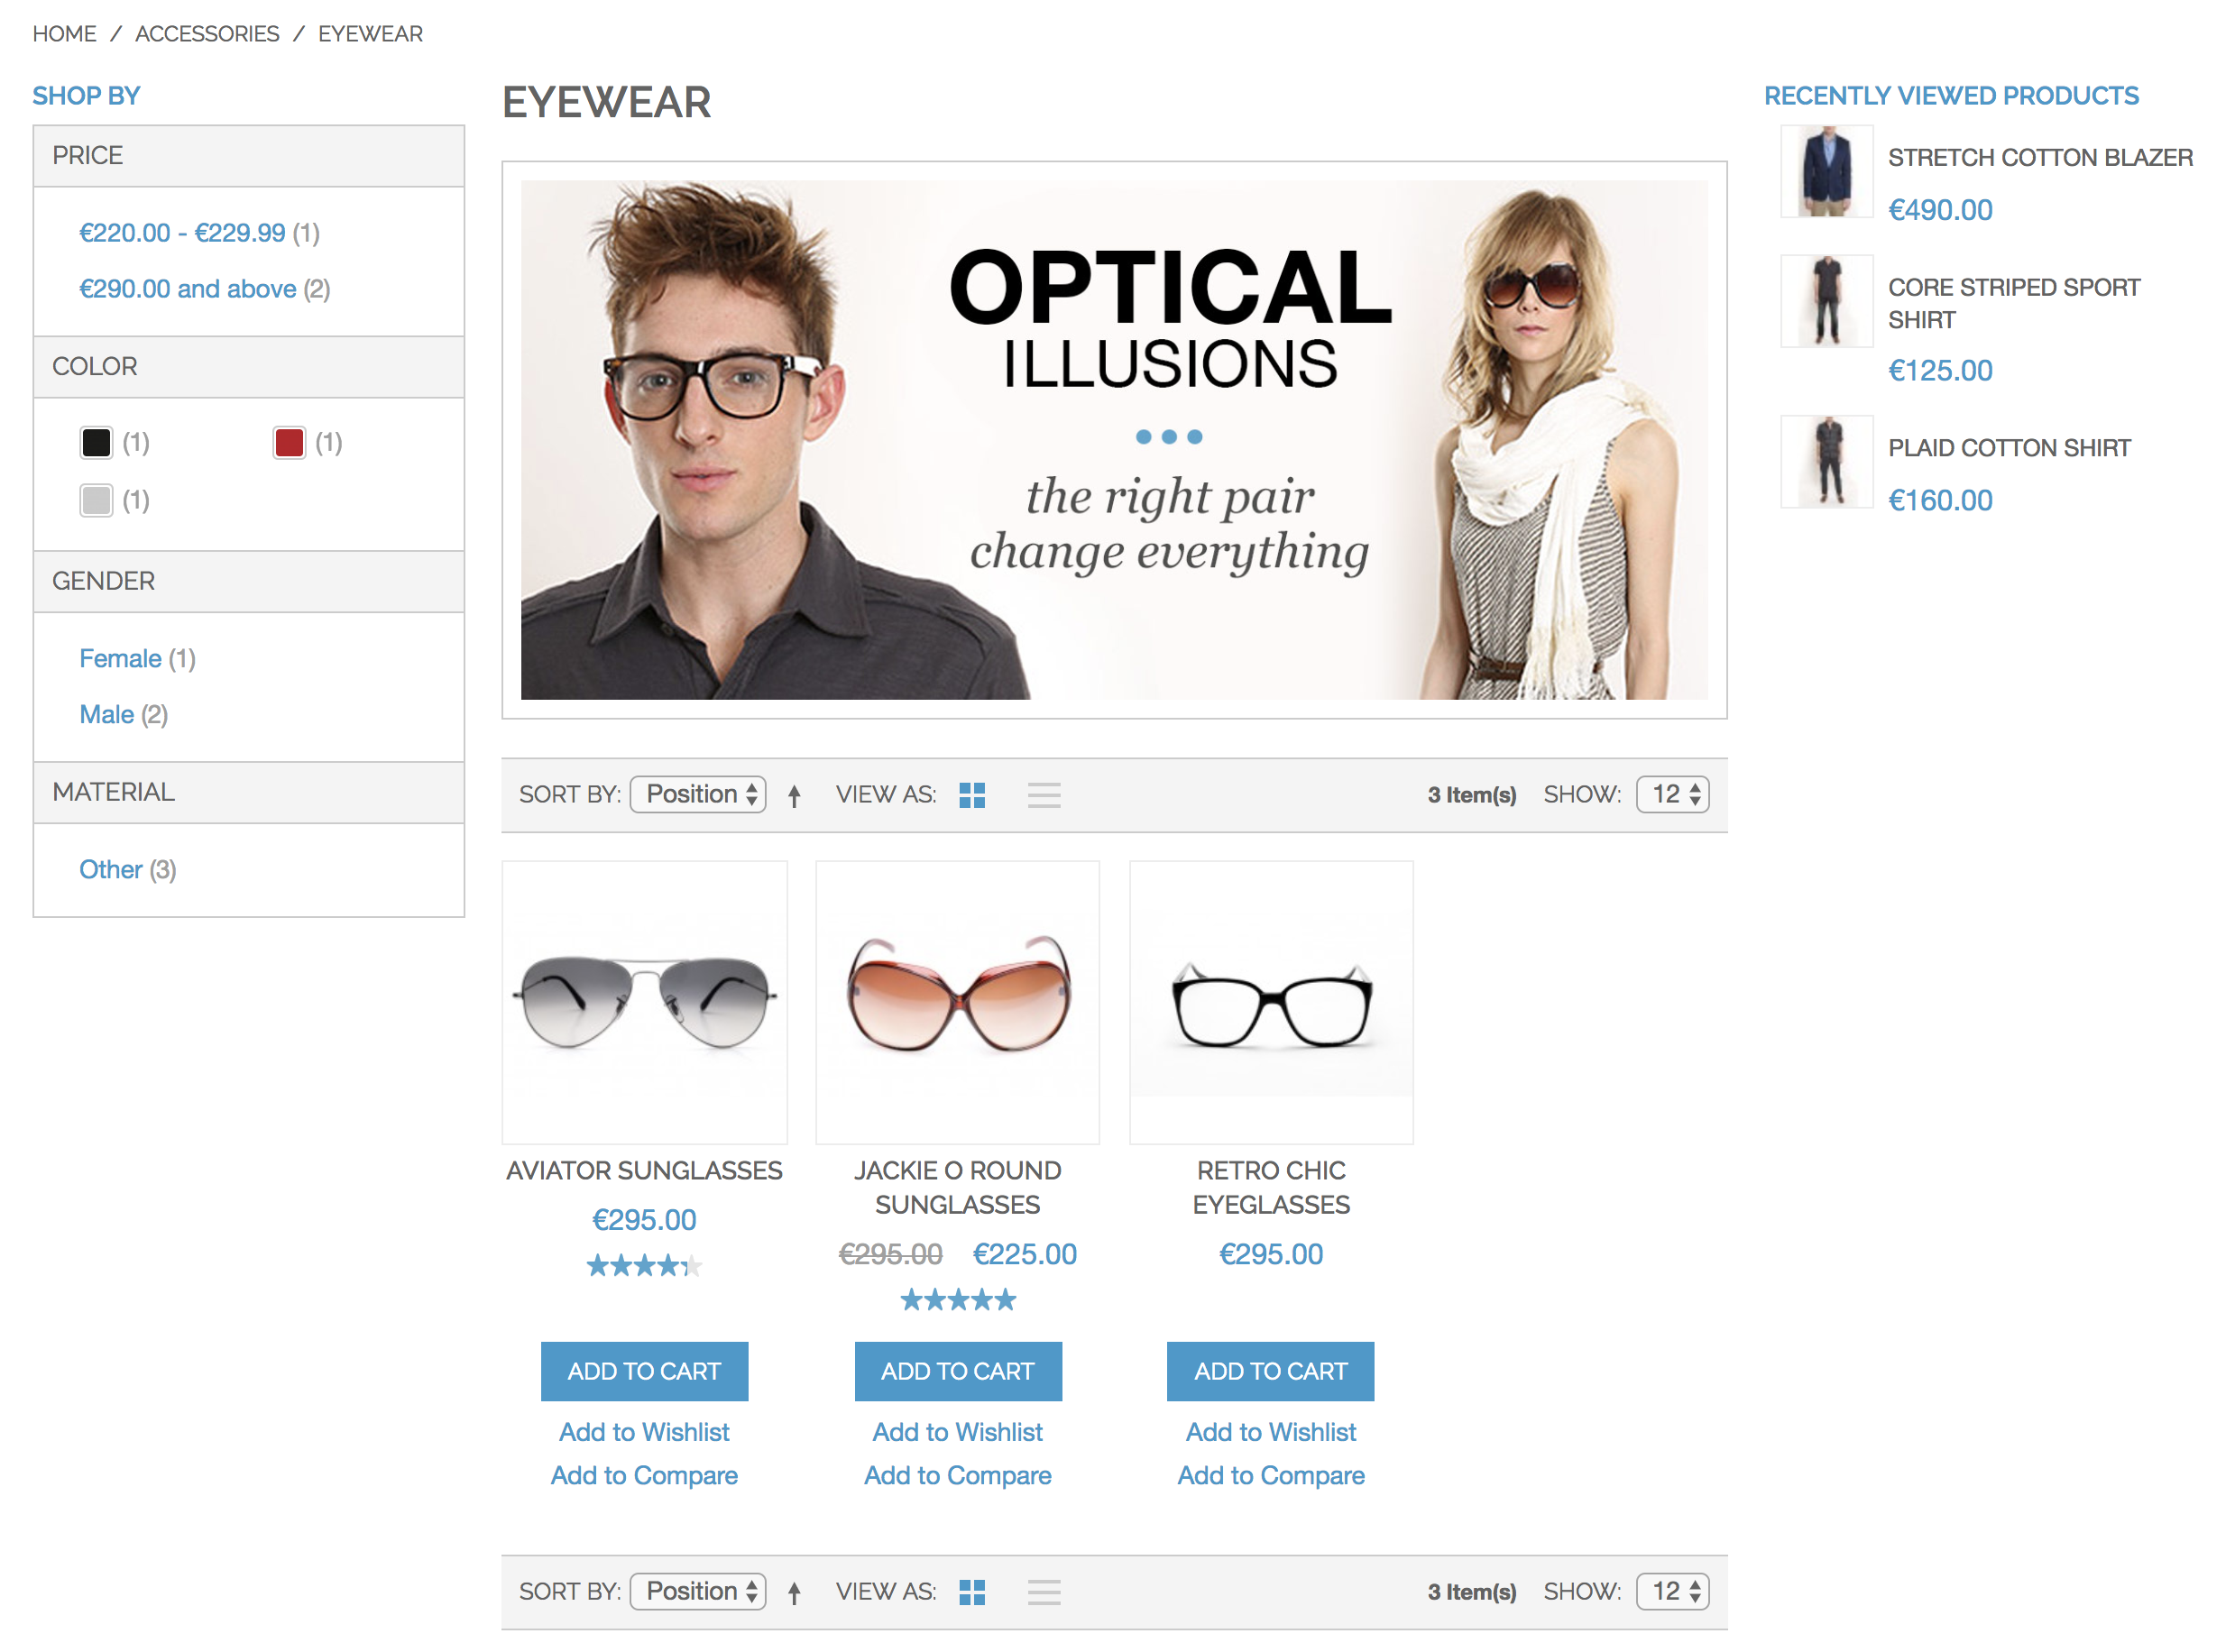
\includegraphics[height=12cm]{images/diagrams/after/desktop-category.png}
  \caption{Updated Category Page Desktop Version}
  \label{fig:desktop-after-category}
\end{figure}
\vspace{0.5cm}

\newpage
\subsection{Product Page}

Differently from the other page enhancements presented so far, the modified web model for the Product Page does not offer any additional visual segments to the page when compared to its starting IFMLModel. As discussed in \ref{product-page-updates}, the change focused on improving the logic behind the related products selection by filtering the items on top of which a browsing correlation was detected. In Figure \ref{fig:desktop-after-product}, we can see an example of this behaviour, where the \textbf{Plaid Cotton Shirt} product is placed as the first one in the Related Products region on the \textbf{Core Striped Sport Shirt} product page.

\vspace{0.5cm}
\begin{figure}[H]
  \centering
    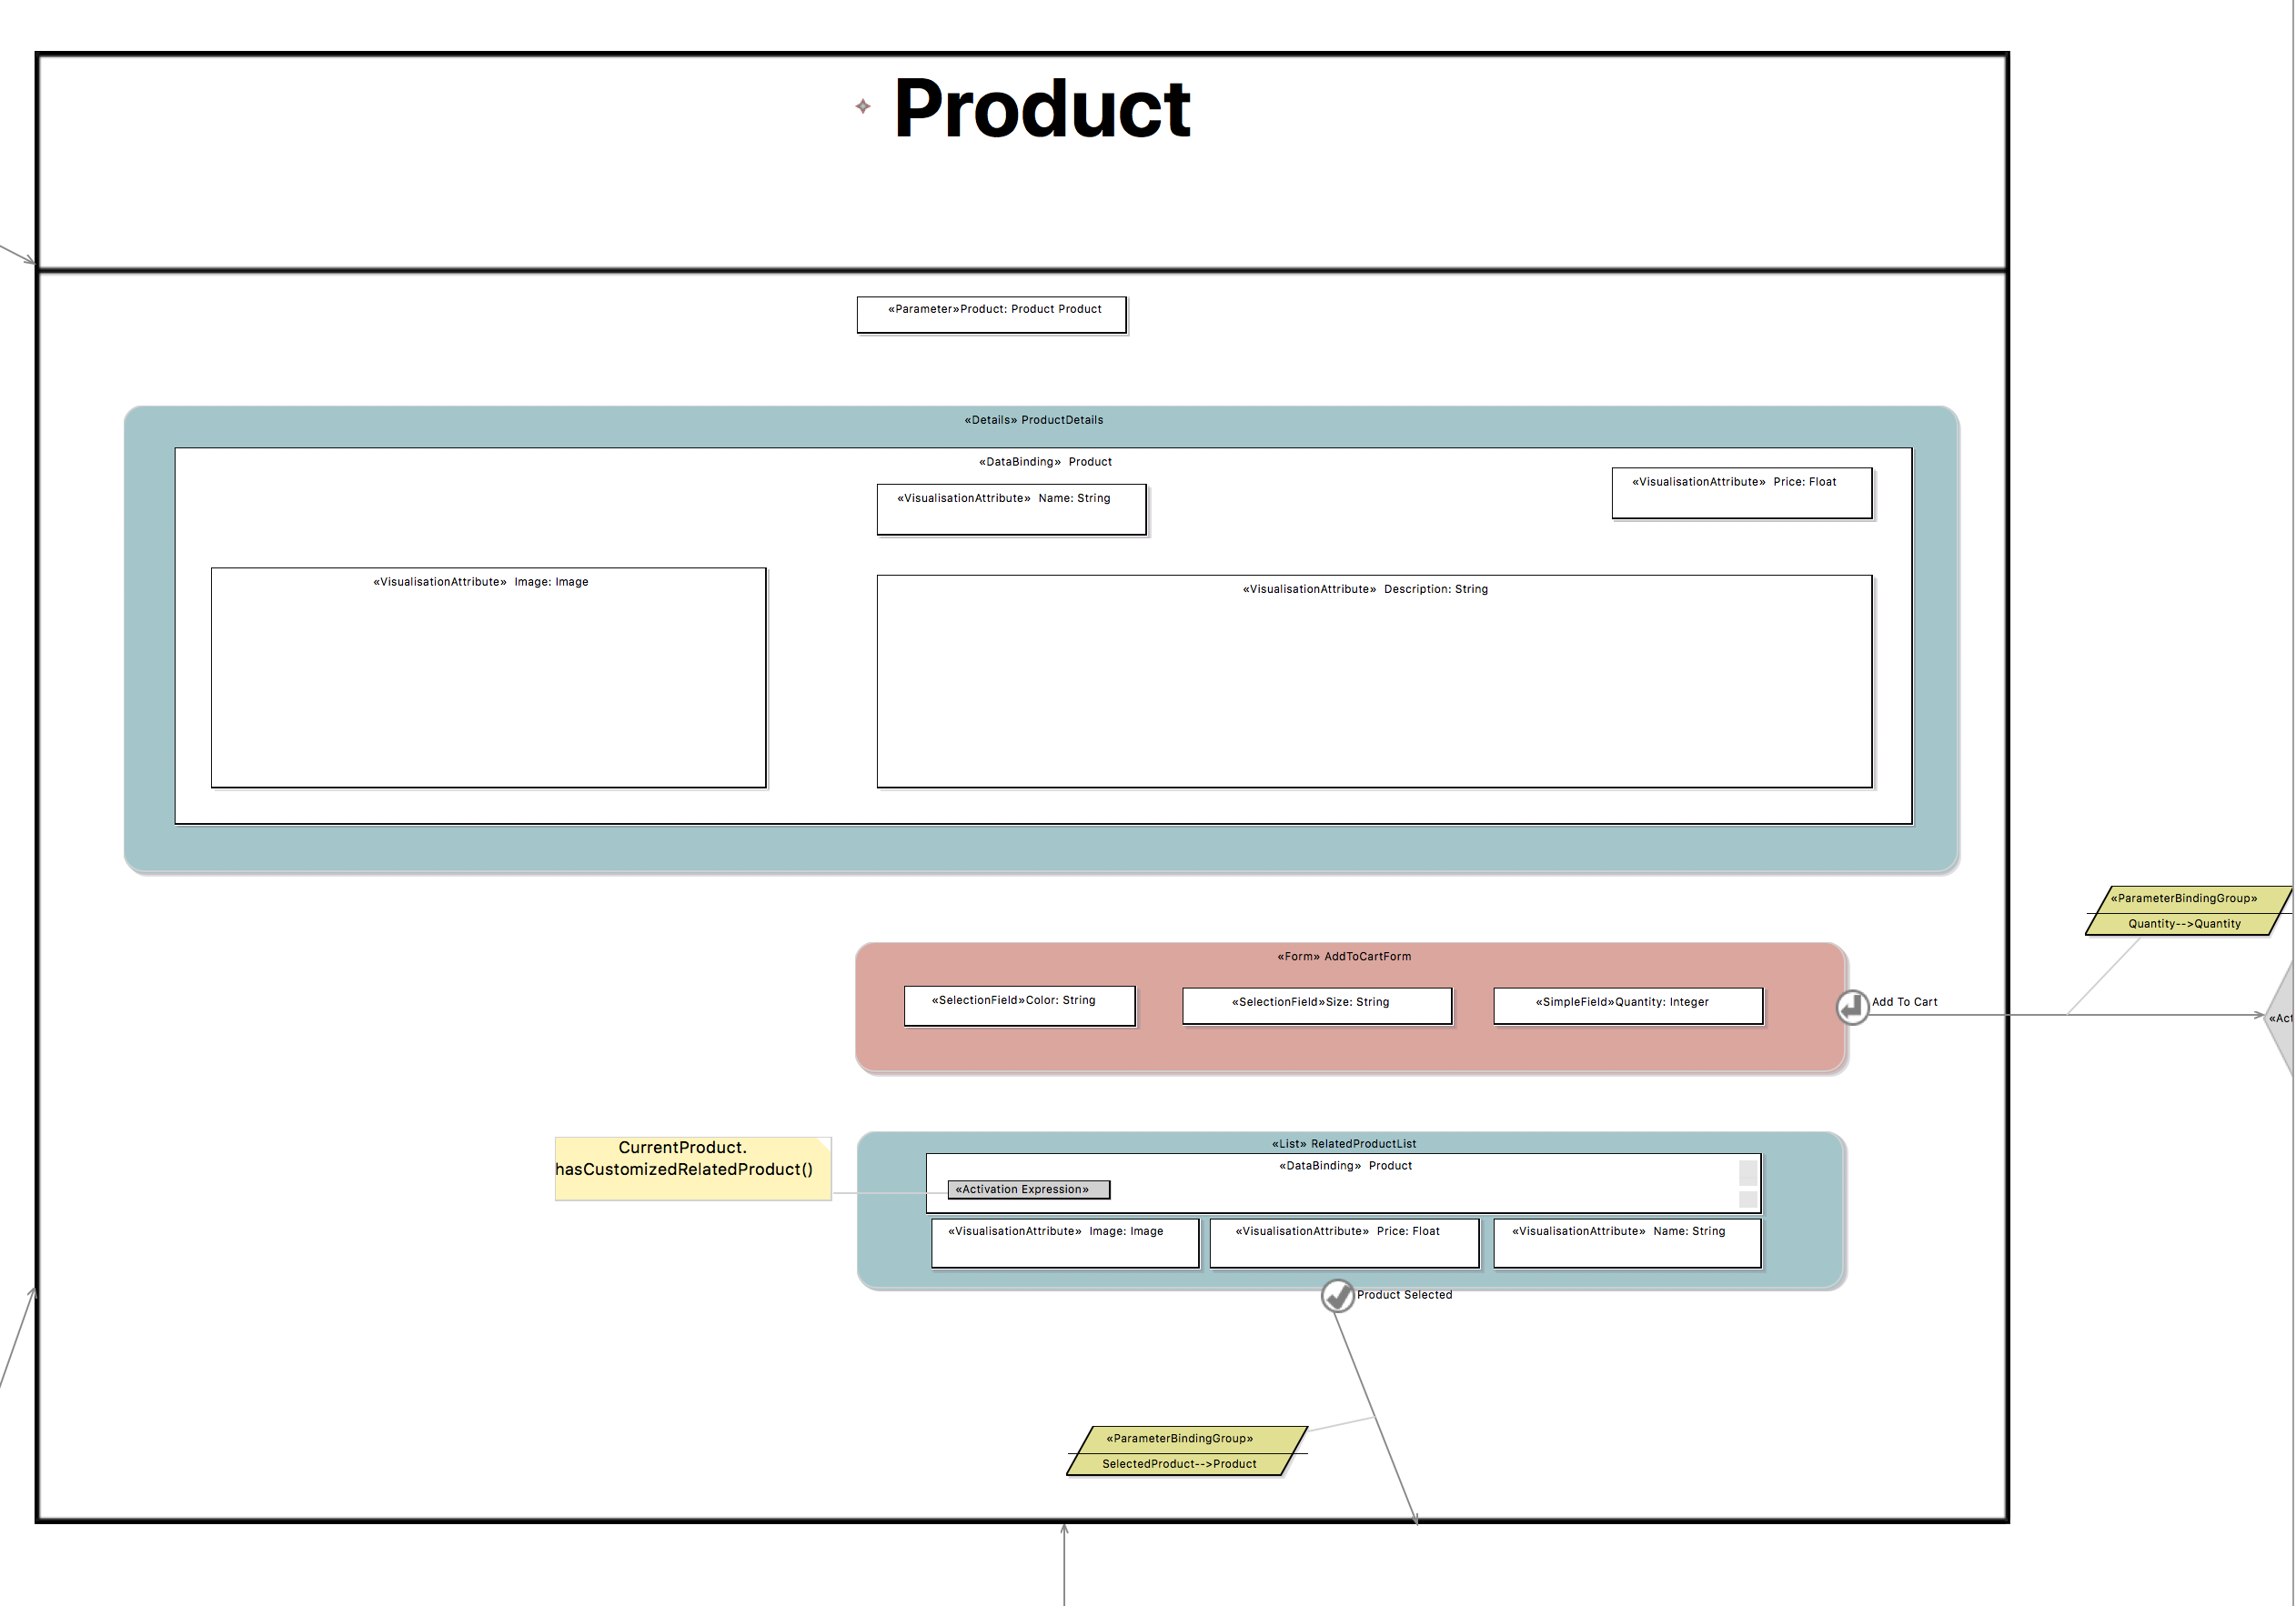
\includegraphics[width=13cm]{images/diagrams/after/ifml-product.png}
  \caption{Updated Product Page IFML Diagram}
  \label{fig:ifml-after-product}
\end{figure}

\begin{figure}[H]
  \centering
    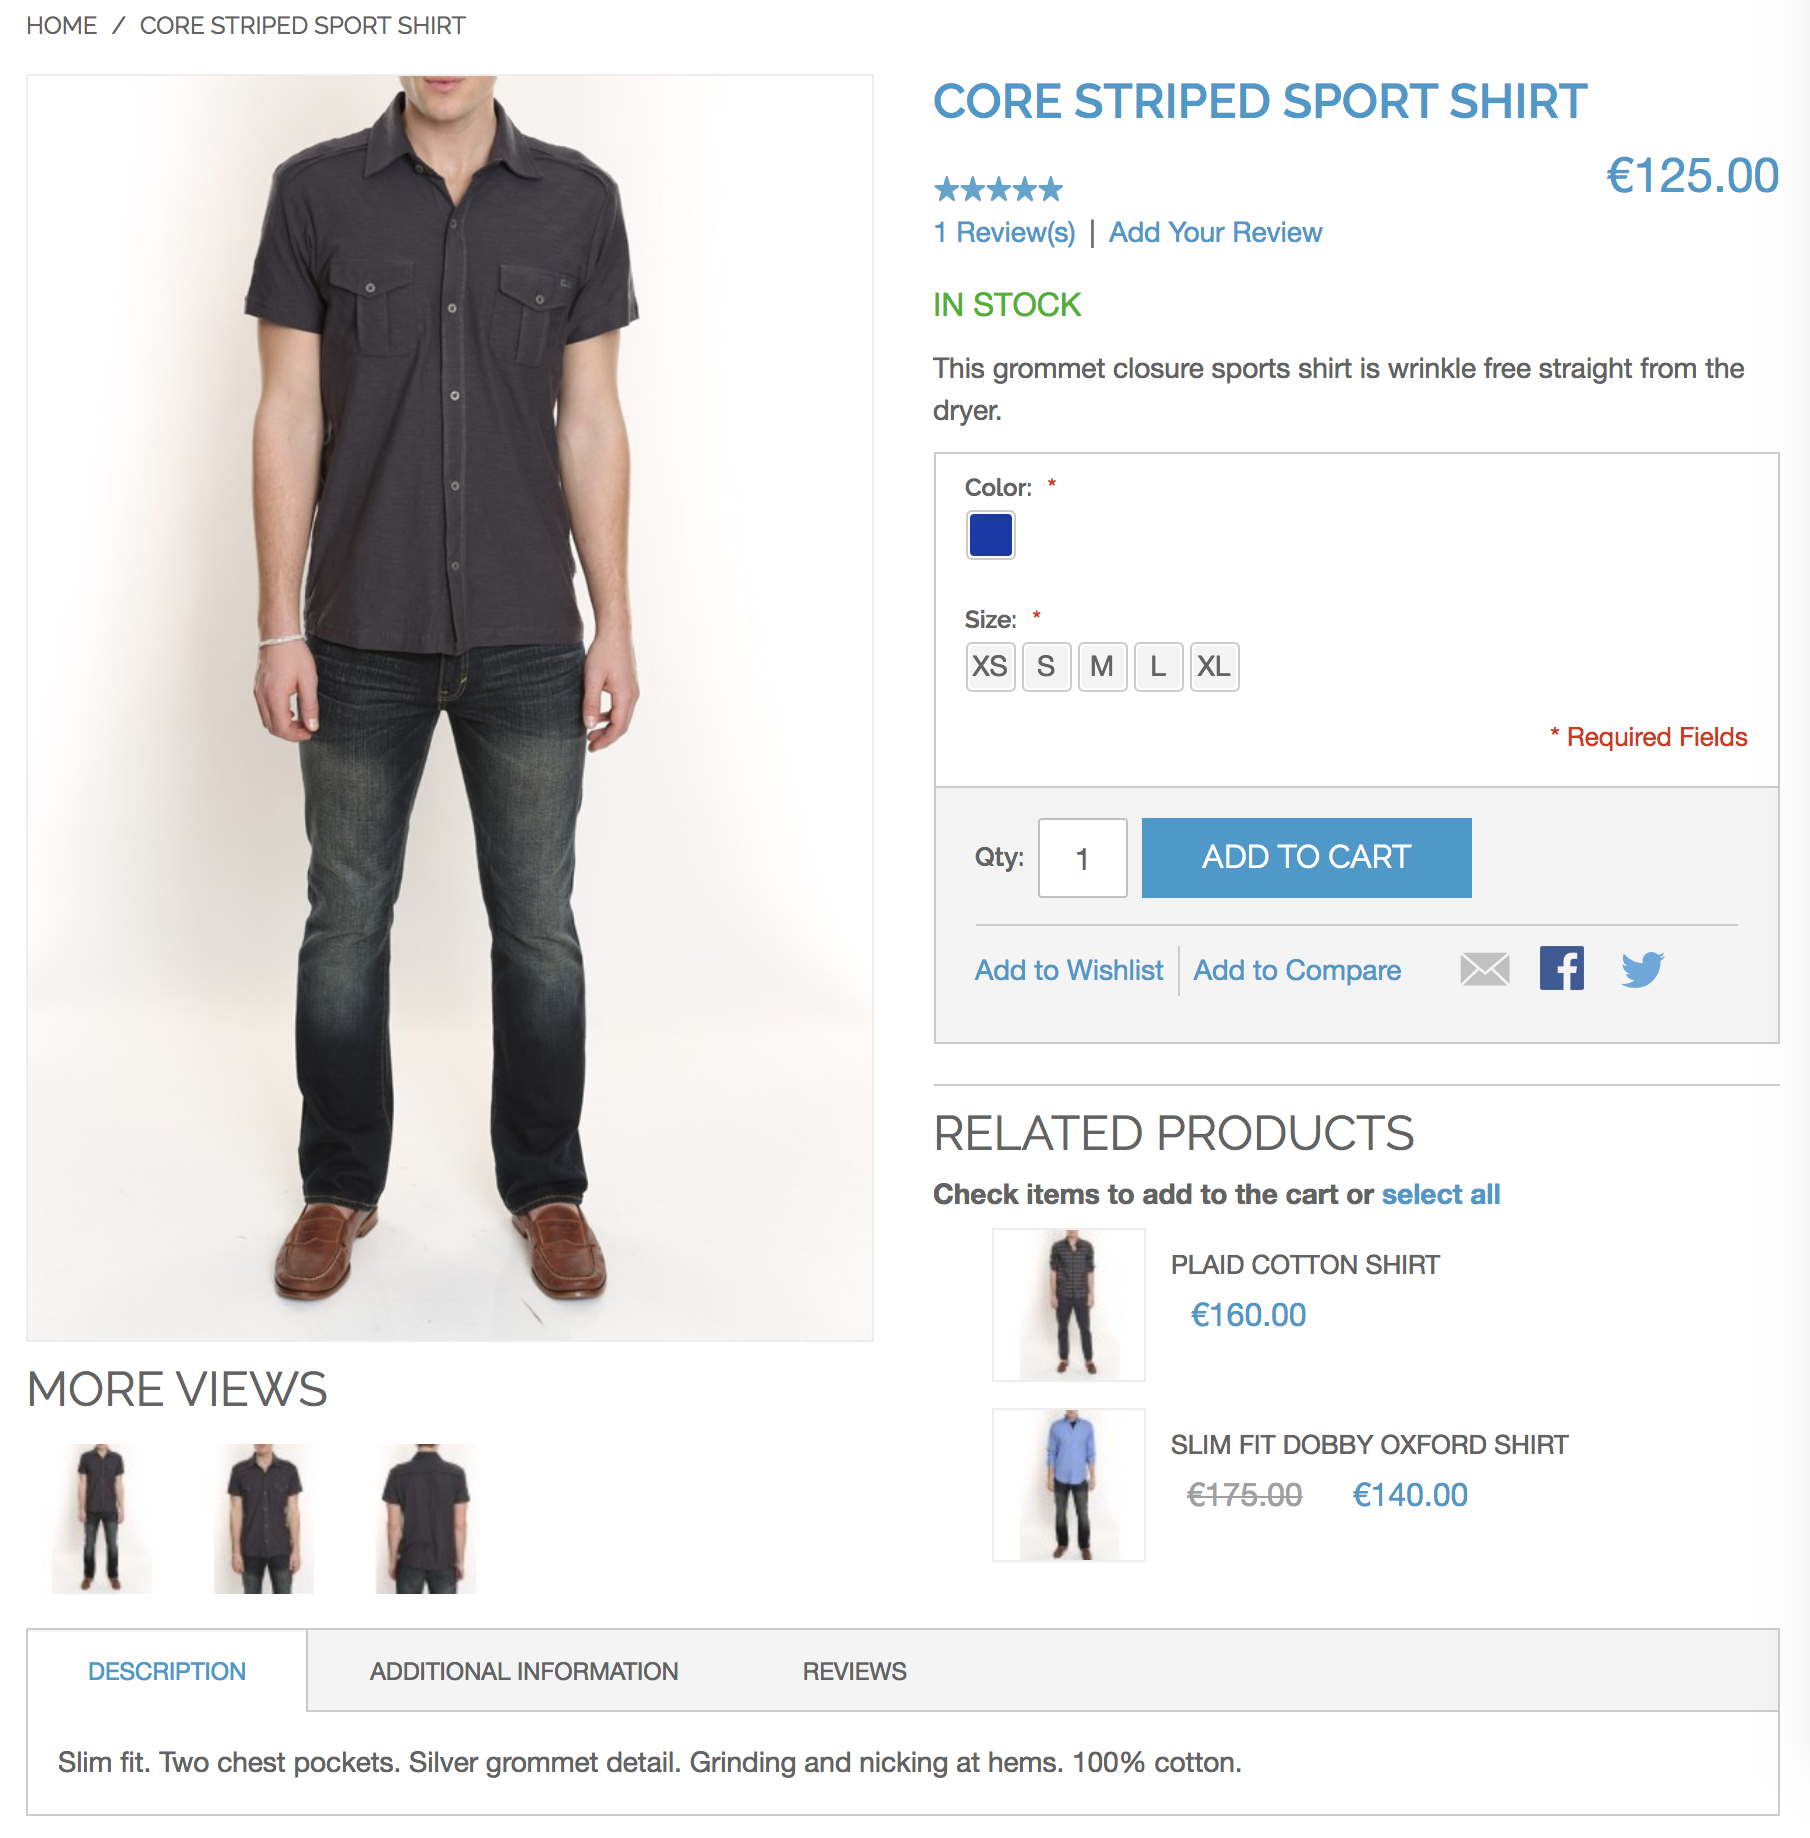
\includegraphics[height=12cm]{images/diagrams/after/desktop-product.png}
  \caption{Updated Product Page Desktop Version}
  \label{fig:desktop-after-product}
\end{figure}
\vspace{0.5cm}

\newpage
\subsection{Shopping Cart}

In \ref{shopping-cart-updates}, we outlined how the visual aspects of the shopping cart sidebar would be transformed through an \textit{IFMLModel} change. This change would result in a new form element within the sidebar, which would be responsible for controlling the application of the reward points available to the customer at that point. Those reward points --- generated through actions recorded as part of the real usage data profiling --- would be converted into discounts that the customer could apply to their current quote at any time. As shown by the attached action in the IFML Diagram, the customer is redirected to the shopping cart page after the discount is applied.

\vspace{0.5cm}
\begin{figure}[H]
  \centering
    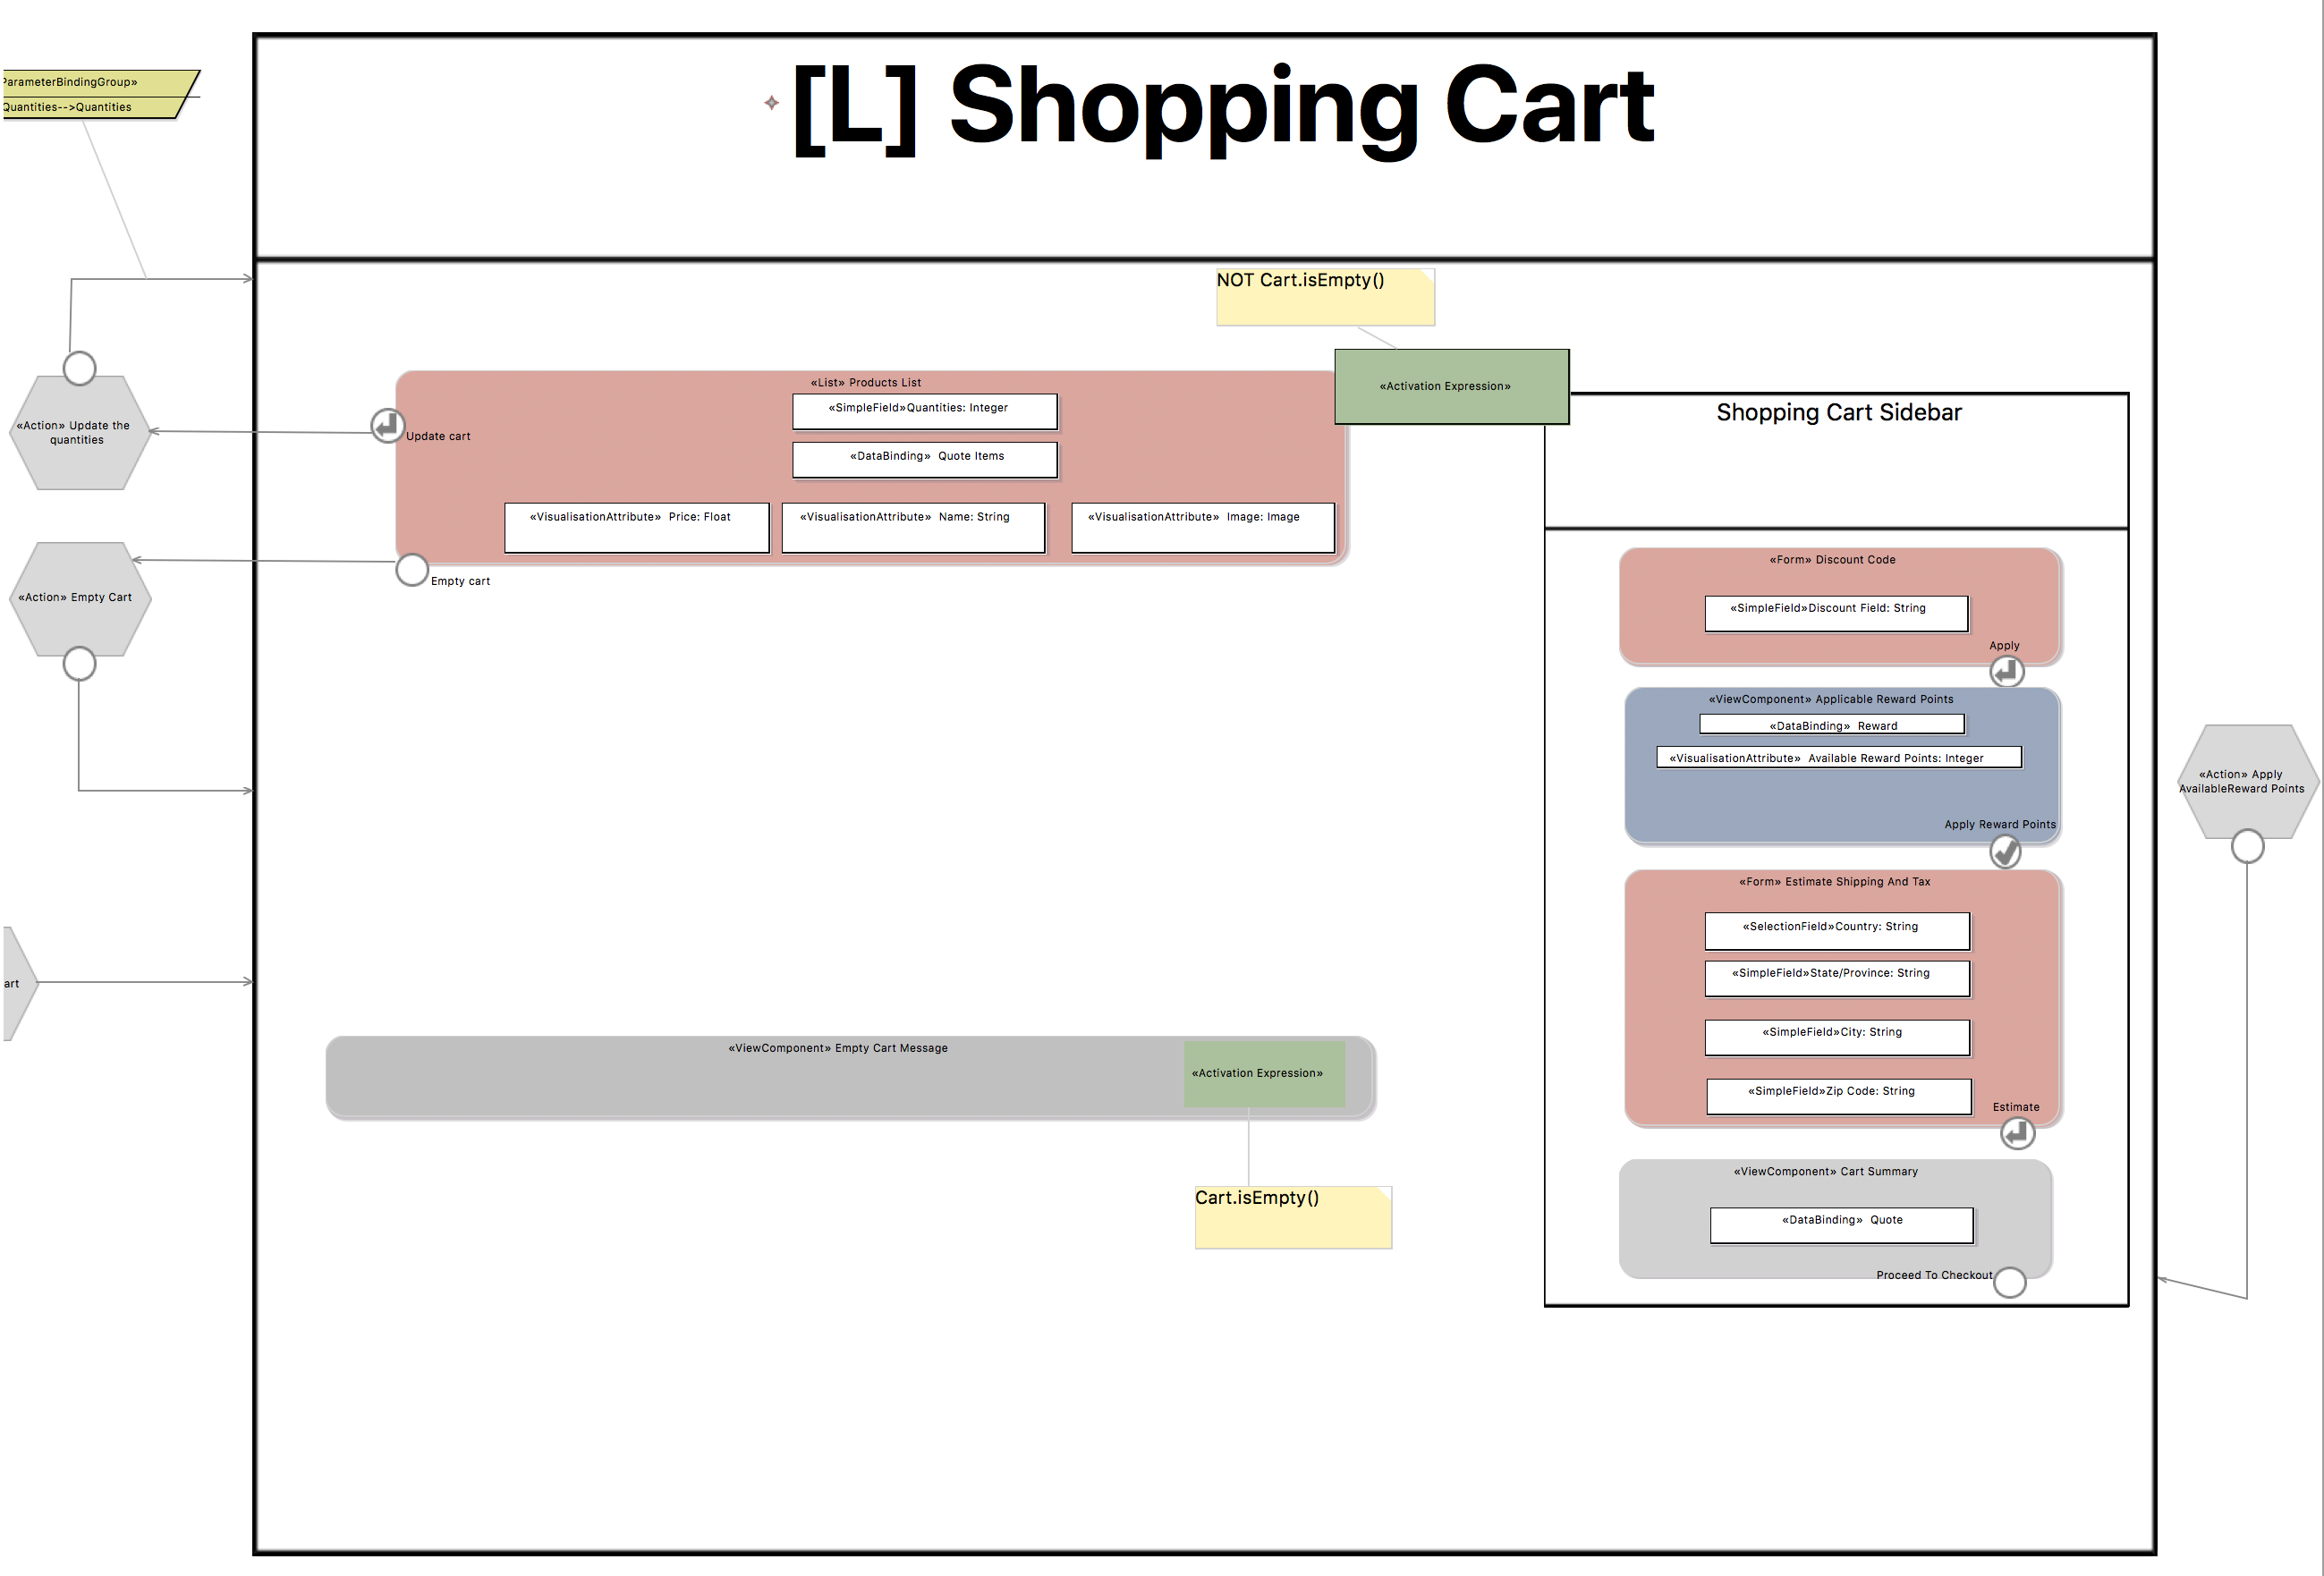
\includegraphics[width=14cm]{images/diagrams/after/ifml-shopping-cart.png}
  \caption{Updated Shopping Cart Page IFML Diagram}
  \label{fig:ifml-after-shopping-cart}
\end{figure}

\begin{figure}[H]
  \centering
    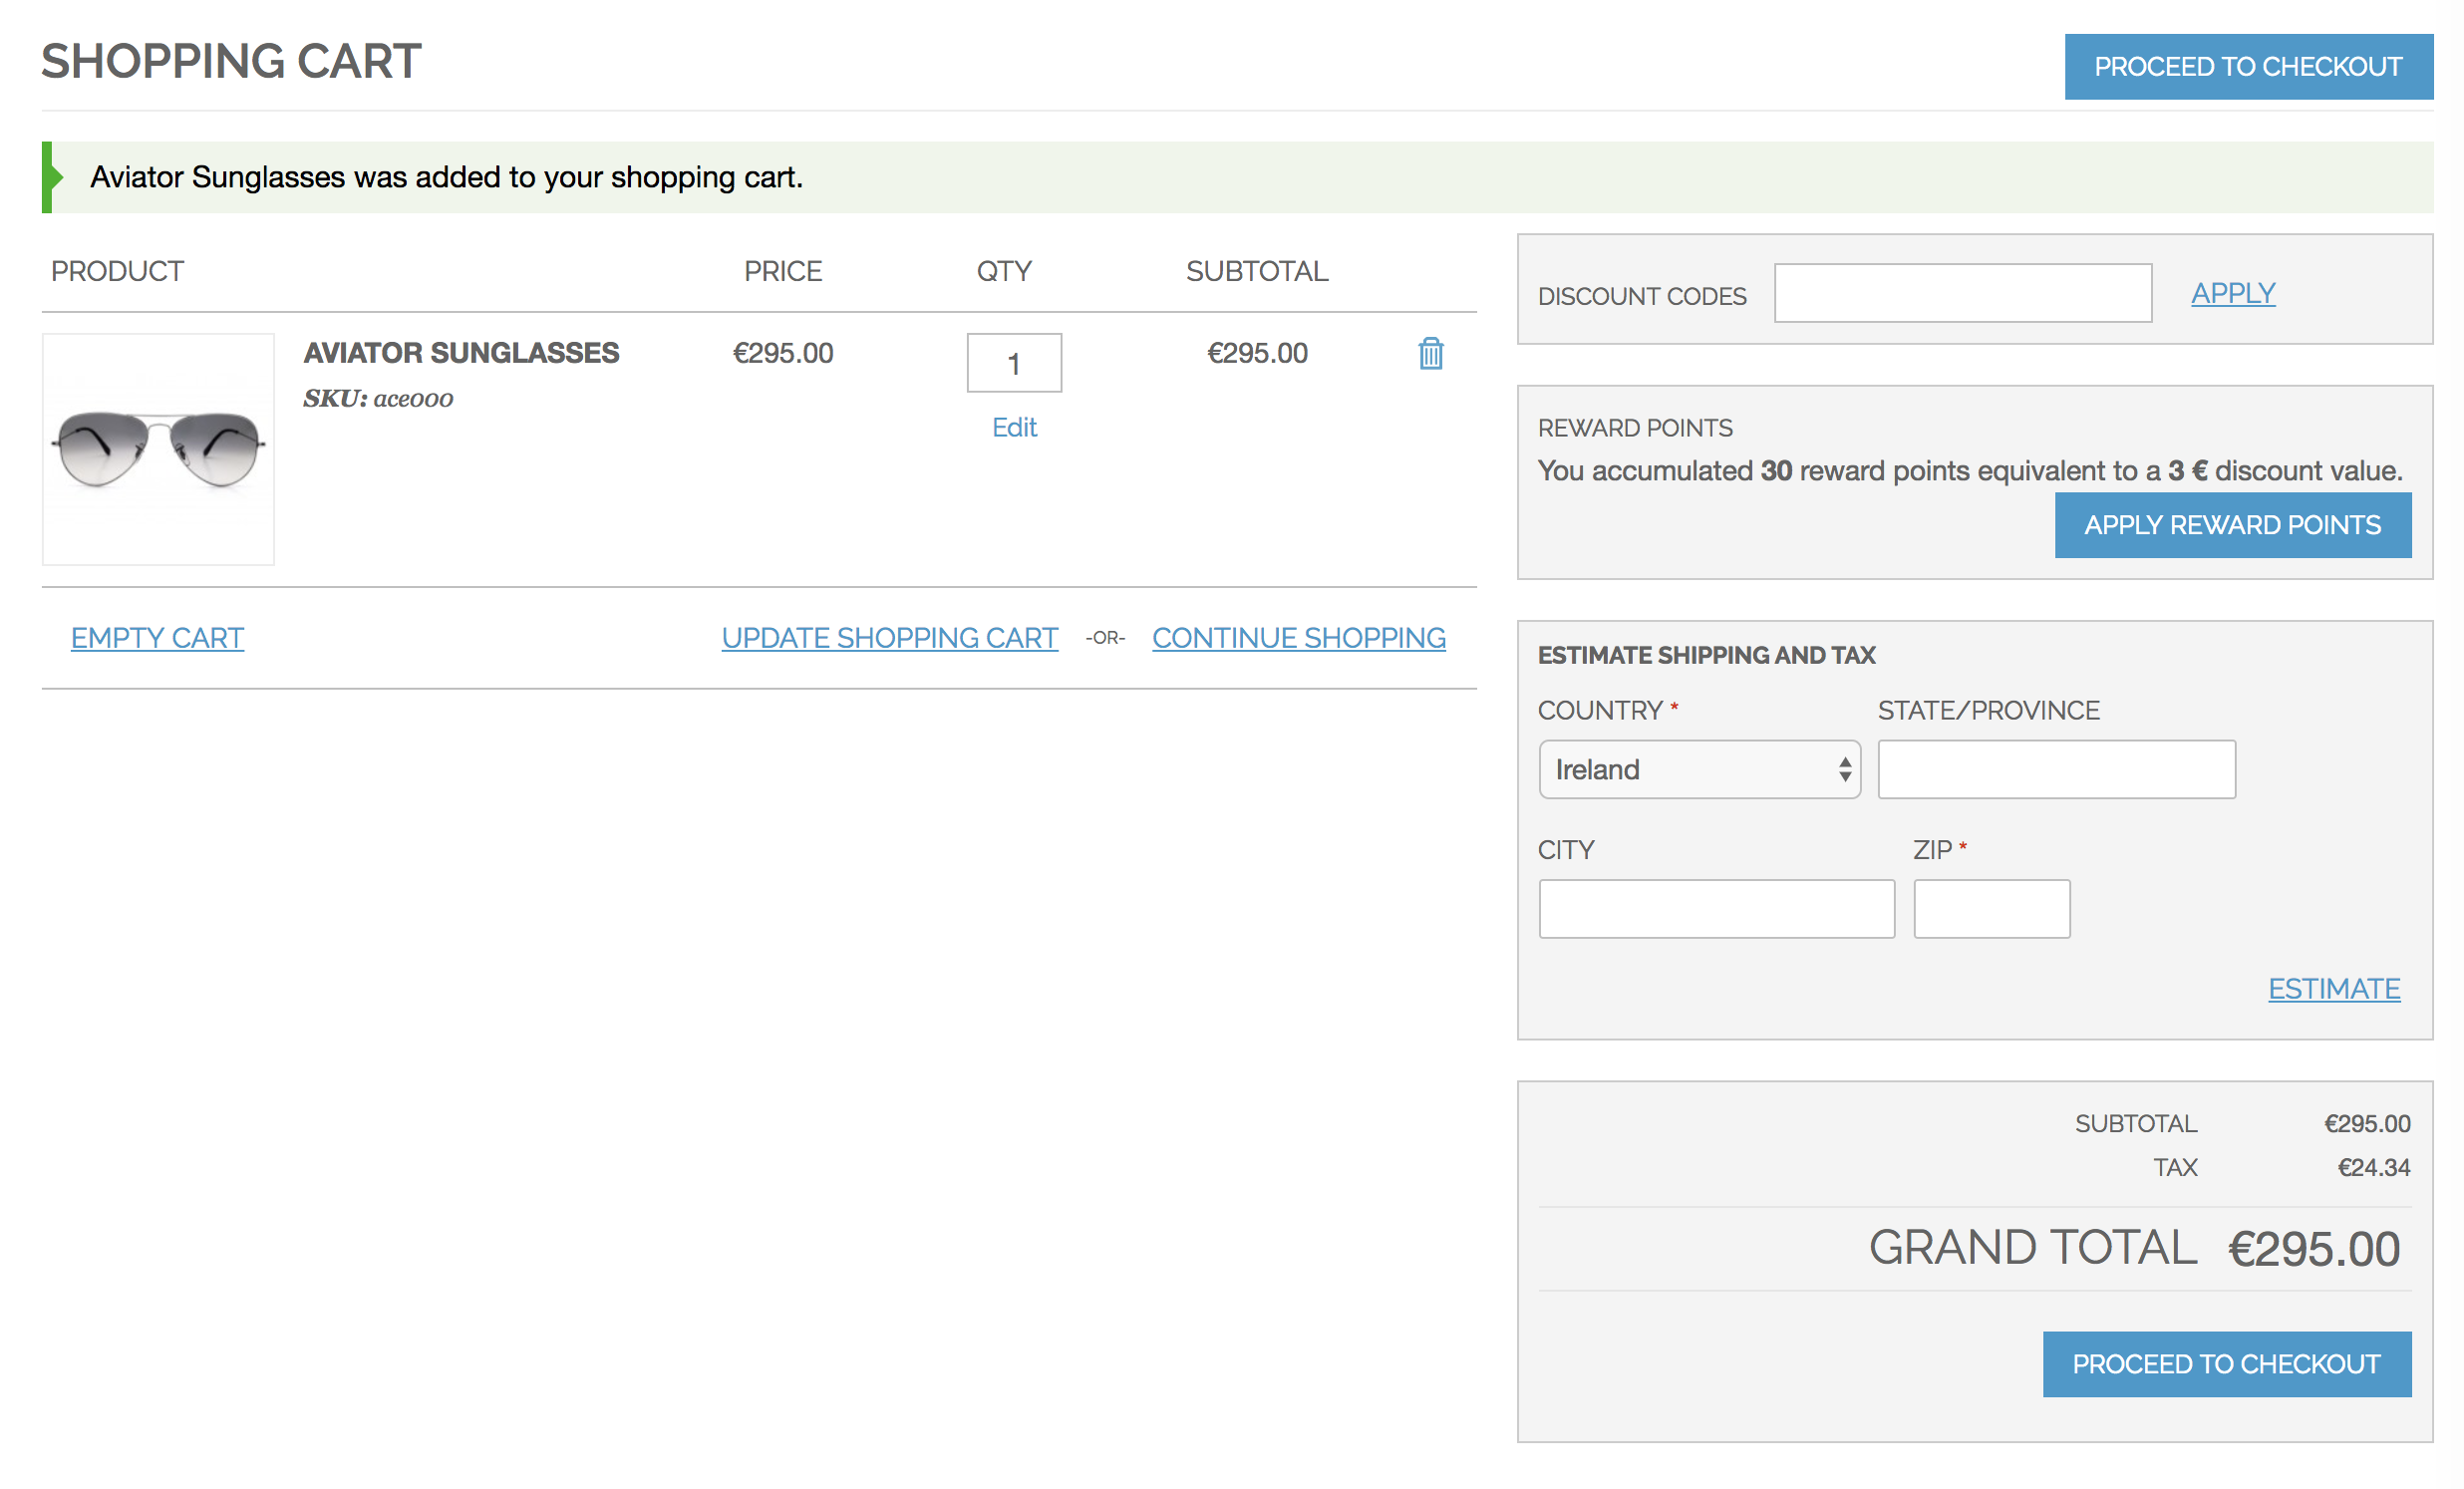
\includegraphics[width=14cm]{images/diagrams/after/desktop-shopping-cart.png}
  \caption{Updated Shopping Cart Page Desktop Version}
  \label{fig:desktop-after-shopping-cart}
\end{figure}
\vspace{0.5cm}

%\addcontentsline{toc}{chapter}{}
